\documentclass[5p,twocolumn,nonatbib,reversenotenum]{elsarticle}

\usepackage[utf8]{inputenc}
\usepackage{amsmath,amssymb}
\usepackage{graphicx}
\usepackage{siunitx}
\usepackage{subcaption}
\usepackage{multirow}
\usepackage{tikz}
\usetikzlibrary{arrows.meta,backgrounds,calc,fit,positioning}
\usepackage[hyphens]{url}
\usepackage[numbers,sort&compress]{natbib}
\usepackage{xspace}
\renewcommand{\bibfont}{\small}
\setlength{\bibsep}{3pt plus 0.3ex}
\usepackage{balance}
\usepackage{placeins}
\usepackage[hidelinks]{hyperref}
\pdfstringdefDisableCommands{\def\corref#1{}}

\newcommand{\methodname}{TopoSIGMA\xspace}
\newcommand{\etalcite}[1]{et al.~\cite{#1}}
\newcommand{\ie}{i.e.,\xspace}
\newcommand{\eg}{e.g.,\xspace}

\journal{Robotics and Autonomous Systems}

\begin{document}
\begin{frontmatter}

\title{\methodname: Spectral Information-Geometric Mapping Architecture}

\author[1]{Manuel Rodriguez-Villegas\corref{cor1}}
\ead{manuelrodriguez@alu.comillas.edu}
\author[2]{Jaime Boal}
\ead{jaime.boal@iit.comillas.edu}
\author[2]{Jesus Tordesillas}
\ead{jtordesillas@comillas.edu}
\cortext[cor1]{Corresponding author}

\affiliation[1]{organization={ICAI School of Engineering, Comillas Pontifical University},
addressline={Alberto Aguilera, 25}, postcode={28015}, postcodesep={}, city={Madrid}, country={Spain}}
\affiliation[2]{organization={Institute for Research in Technology~(IIT), ICAI School of Engineering, Comillas Pontifical University},
addressline={Rey Francisco, 4}, postcode={28008}, postcodesep={}, city={Madrid}, country={Spain}}

\begin{abstract}
    Topological maps represent an environment as places and connections between them. We present \methodname, an online visual topological mapper that uses frozen image descriptors without task-specific training. An adaptive detector identifies node boundaries from changes in the spectral connectivity of recent observations. Each node is represented by a von Mises--Fisher distribution, which describes both its main appearance and the variation among its views. For loop closure, an odometry-based uncertainty budget restricts the candidate set, and bidirectional visual sequences distinguish between multiple compatible places. Across seven indoor traversals, the complete system accepted 25 correct and two incorrect loop closures at a 2 m evaluation tolerance. Relative to geometry-only association, visual validation increased precision from 0.829 to 0.926, while reducing recall from 0.604 to 0.521. Adaptive boundary detection produced more consistent node creation rates than fixed prominence and higher loop closure scores at all four evaluated tolerances. Comparisons with an AnyLoc-inspired descriptor and multi-view cosine validation depended on the environment and evaluation tolerance. These results support geometric restriction and selective visual validation when avoiding incorrect connections is more important than recovering every revisit.
\end{abstract}

\begin{keyword}
Visual Topological Mapping \sep Loop Closure \sep Spectral Graph \sep Information Geometry \sep Vision Foundation Model \sep Text-to-Node Retrieval
\end{keyword}

\end{frontmatter}

\section{Introduction}
Autonomous robots need maps that support localization and navigation. Metric Simultaneous Localization and Mapping (SLAM) estimates landmarks, surfaces or occupancy grids~\cite{Cadena2016SLAM}, providing the geometry needed for local motion and obstacle avoidance. A topological map describes the environment at a coarser level: nodes represent places, and edges record connections between them. Building this graph requires deciding when observations belong to a new place and when they revisit an earlier one. \methodname addresses these two decisions using monocular images to describe appearance and planar odometry to constrain revisit associations.

Several systems combine geometric and topological representations. Topomap extracts navigable topology from sparse visual-SLAM landmarks, hierarchical semantic maps organize recognized content at several spatial scales, and situational graphs represent places, objects and rooms in 3D~\cite{Blochliger2018,Luo2018,Bavle2022}. RTAB-Map uses short- and long-term memory to manage appearance-based mapping as experience grows~\cite{Labbe2019RTABMap}. These approaches support richer map representations than a graph of visual segments alone. For applications that need such a graph without reconstructing the full scene, \methodname builds nodes directly from the image stream and uses recorded odometry for spatial context.

Visual representation affects both node creation and revisit recognition. FAB-MAP models the probability that an observation belongs to a known place while accounting for perceptual aliasing~\cite{Cummins2008FABMAP}. Later work incorporates deep features into topological-semantic maps~\cite{Sousa2022}, and AnyLoc uses self-supervised transformer features for visual place recognition across diverse environments~\cite{Keetha2023AnyLoc}. A descriptor that retrieves similar images, however, does not by itself specify where to place graph nodes or which matches should become edges. We use frozen DINOv2 descriptors~\cite{oquab2024dinov2learningrobustvisual} within an explicit node-creation and association procedure, and evaluate an AnyLoc-inspired alternative through that same procedure.

Node selection determines what a place means in the map. Geometric rules can align nodes with landmarks or free-space structure~\cite{Blochliger2018}, while Neural Topological SLAM and learned graph memories select representations for downstream navigation~\cite{Chaplot2020NeuralTopo,Kwon2021,Kim2023}. Appearance-based segmentation offers a training-free alternative, but a fixed detection scale may split a visually varied room too often or miss changes in a repetitive corridor. Spectral graph quantities describe how a set of observations groups together~\cite{Fiedler1973,Chung1997,vonLuxburg2007}, and Boal and S\'anchez-Miralles use algebraic connectivity for online visual segmentation~\cite{Boal2016}. Building on that principle, \methodname uses non-negative descriptor similarities and scales the required recovery from each connectivity valley to recent signal variation.

Loop closure must distinguish a revisit from a different place with similar doors, furniture or corridor structure~\cite{Lowry2016VPR}. SeqSLAM uses coherent visual sequences to handle large appearance changes~\cite{Milford2012SeqSLAM}. Other systems combine appearance with geometric evidence: Hydra optimizes a 3D scene graph, H-SLAM combines direct and indirect visual constraints, and PRISM-TopoMap verifies place recognition through point-cloud registration~\cite{Hughes2022,Younes2024,muravyev2025prism}. \methodname applies a simpler spatial check suited to RGB images and planar odometry: an accumulated uncertainty budget defines compatible earlier nodes, and visual sequences distinguish between them when several remain.

A further question is how to compare a node containing several views. A mean descriptor captures its central appearance but cannot distinguish closely agreeing observations from a broad spread of views. Directional statistics describe both properties for unit-length vectors~\cite{Mardia2000Directional}. We therefore fit a von Mises--Fisher (vMF) distribution to each node's normalized descriptors. Its mean records the main appearance and its concentration records how consistently that appearance was observed. Distribution overlap then supplies the evidence for sequence comparison.

The retained views also support a secondary application. We use the Contrastive Language-Image Pre-training (CLIP) model to place text and images in a shared representation~\cite{radford2021learningtransferablevisualmodels}, and then rank graph nodes for requests such as ``take me to the kitchen.'' This connects language queries to the visual places already stored by the mapper, and we evaluate room-class retrieval with 100 queries on four annotated maps.

\methodname makes the following contributions:
\begin{itemize}
    \item an adaptive node-boundary detector that extends algebraic-connectivity segmentation with non-negative visual affinities and a prominence threshold based on recent signal variation;
    \item a loop closure architecture that combines an odometry-based uncertainty budget with bidirectional vMF sequence comparison when several spatial candidates remain;
    \item a controlled evaluation of node creation, loop association and descriptor choice across seven indoor traversals and four spatial tolerances, separating loop edges from sequential connectivity.
\end{itemize}

The implementation and experiments are publicly available at \url{https://github.com/manuel-rodriguezvillegas/topo_sigma}.

\begin{figure*}[t]
    \centering
    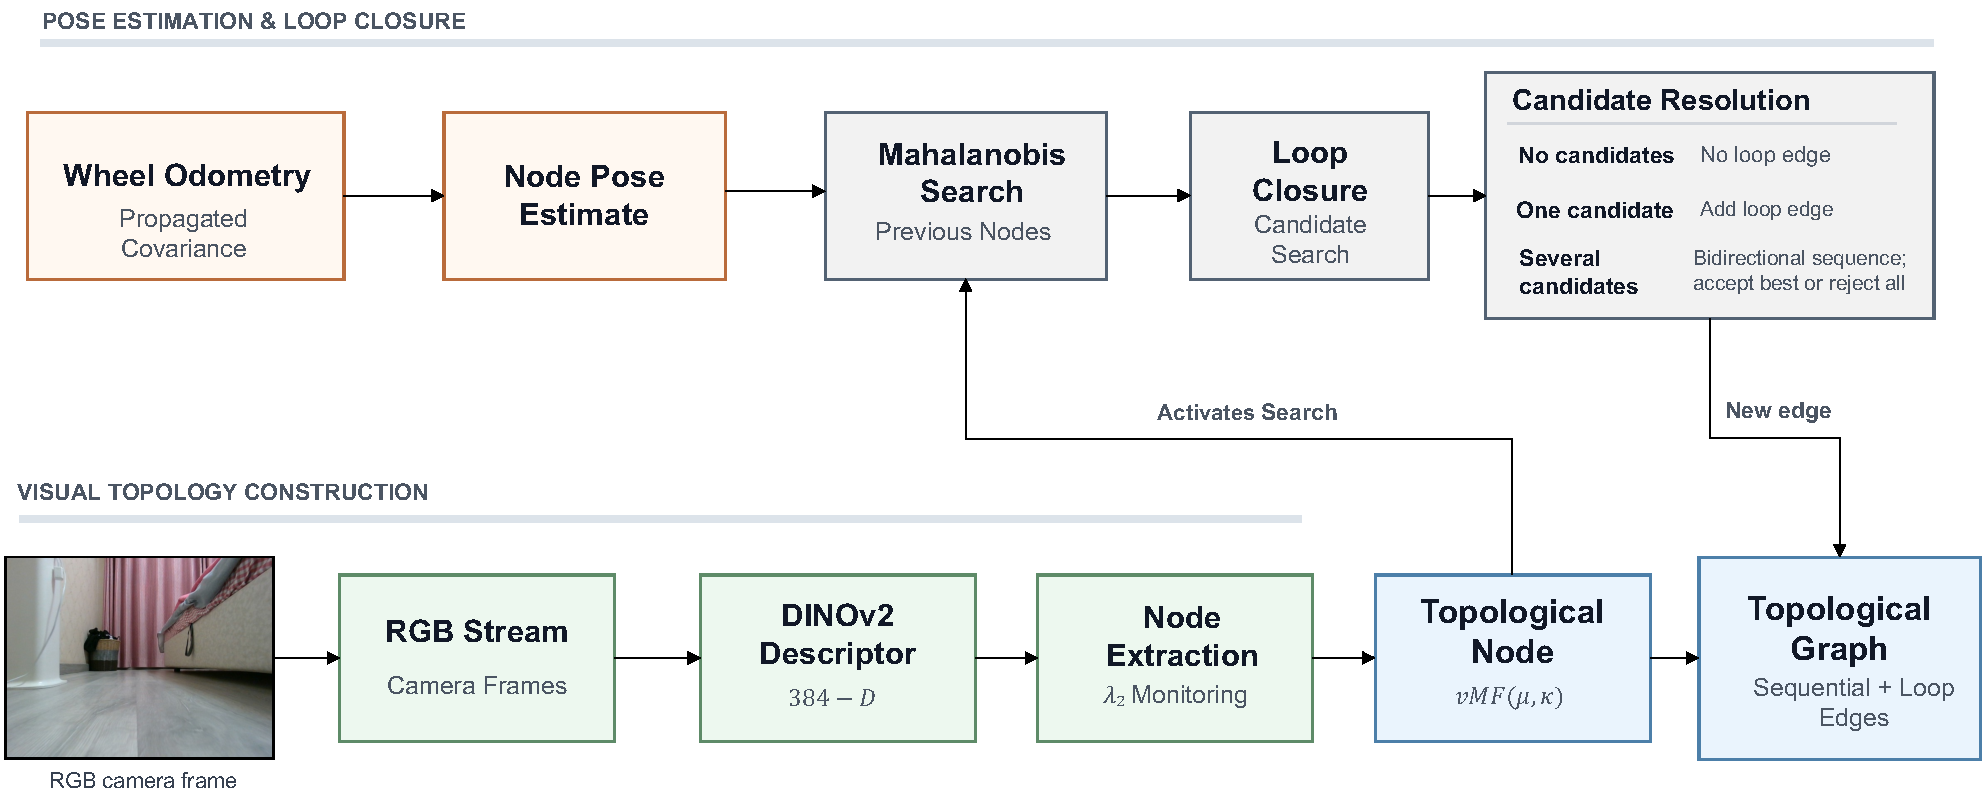
\includegraphics[width=\textwidth]{images/whole_process.pdf}
    \caption{Complete online mapping pipeline. DINOv2~\cite{oquab2024dinov2learningrobustvisual} descriptors form a recent similarity graph whose algebraic connectivity $\lambda_2$ supplies node boundaries. Each completed segment is represented by a vMF distribution and connected sequentially. The wheel-odometry budget creates a compatible revisit set: if there are no candidates, the route continues; one adds a loop edge directly, and several trigger a bidirectional vMF sequence comparison before the graph is updated.}
    \label{fig:whole_process}
\end{figure*}

\section{Methodology}
Figure~\ref{fig:whole_process} summarizes the mapper. Its output is a graph $G=(V,E)$ in which each node represents a visual segment of the journey. Sequential edges record passage between consecutive segments, while loop edges record accepted revisit associations. Nodes remain separate after a loop is added, as the system does not merge them or optimize their poses.

\subsection{System inputs}
At each step, the mapper receives a synchronized RGB image and a planar odometric pose $(x,y,\theta)$. The image describes the robot's current visual surroundings, while odometry provides the estimated position and motion along the route.

The dataset adapters maintain a cumulative uncertainty budget from the recorded motion that estimates how much we should distrust the recorded odometry. Let $\Delta\ell_t$ be the distance between consecutive planar positions and $\Delta\theta_t$ the heading change wrapped to $[-\pi,\pi)$. Starting from $B_0=0$, the update is
\begin{equation}
\label{eq:motion-budget}
\begin{aligned}
    u_t &= \alpha_3\Delta\ell_t+\alpha_4|\Delta\theta_t|,\\
    v_t &= \alpha_1|\Delta\theta_t|+\alpha_2\Delta\ell_t,\\
    B_t &= B_{t-1}+\operatorname{diag}(u_t,u_t,v_t).
\end{aligned}
\end{equation}
Here $u_t$ adds the same uncertainty to both position axes ($x$ and $y$), and $v_t$ adds angular uncertainty. Longer travel and larger turns therefore increase the budget. The \(\alpha_i\) parameters convert an amount of motion into an increase in variance. Therefore, their units are, respectively, $\mathrm{rad}^2/\mathrm{rad}$, $\mathrm{rad}^2/\mathrm{m}$, $\mathrm{m}^2/\mathrm{m}$ and $\mathrm{m}^2/\mathrm{rad}$. The model does not propagate heading uncertainty into position, and only $(x, y)$ are used for loop closure. Each completed node stores the pose and budget at its representative frame.

\subsection{Node extraction}
\label{sec:node-extraction}
Each frame is encoded by a frozen DINOv2~\cite{oquab2024dinov2learningrobustvisual} small Vision Transformer with 14-pixel patches (ViT-S/14). For frame $k$, let $\mathbf{f}_k\in\mathbb{R}^{384}$ be the resulting descriptor. Normalizing it gives
\begin{equation}
    \mathbf{x}_k=\frac{\mathbf{f}_k}{\lVert\mathbf{f}_k\rVert}.
\end{equation}
The dot product $\mathbf{x}_i^\top\mathbf{x}_j$ is then their cosine similarity.

The mapper must now decide when the current place has changed enough to start a new node. For this we form a weighted graph with the latest $n=30$ descriptors: frames are its vertices, and edge scores depend on their similarities. The affinity matrix $A$ stores these similarities, and the diagonal degree matrix $D$ stores their row sums:
\begin{equation}
    a_{ij}=\begin{cases}
    \max(0,\mathbf{x}_i^\top\mathbf{x}_j), & i\neq j,\\
    0, & i=j,
    \end{cases}
    \qquad d_{ii}=\sum_j a_{ij}.
\end{equation}
Negative cosine values are set to zero because they express disagreement, not a connection. As $D=\operatorname{diag}(d_{ii})$ contains the total edge weight of each frame, the symmetric normalized graph Laplacian is~\cite{Chung1997,vonLuxburg2007}
\begin{equation}
    L_{\mathrm{sym}}=I-D^{-1/2}AD^{-1/2}.
\end{equation}
If a frame has no positive connection, its inverse degree is taken as zero. The second-smallest eigenvalue $\lambda_2$ of this matrix is called the algebraic connectivity~\cite{Fiedler1973,Chung1997}. A high value indicates a well-connected group of recent observations, and a low value indicates that the graph can separate into groups with weak connections between them. During a transition, old and new appearances share the window but connect weakly to one another, so $\lambda_2$ falls and then rises once the new view dominates. Therefore, the bottom of that valley is a natural boundary between nodes. Figure~\ref{fig:ac_pipeline} illustrates this transition.

\begin{figure}[!htbp]
    \centering
    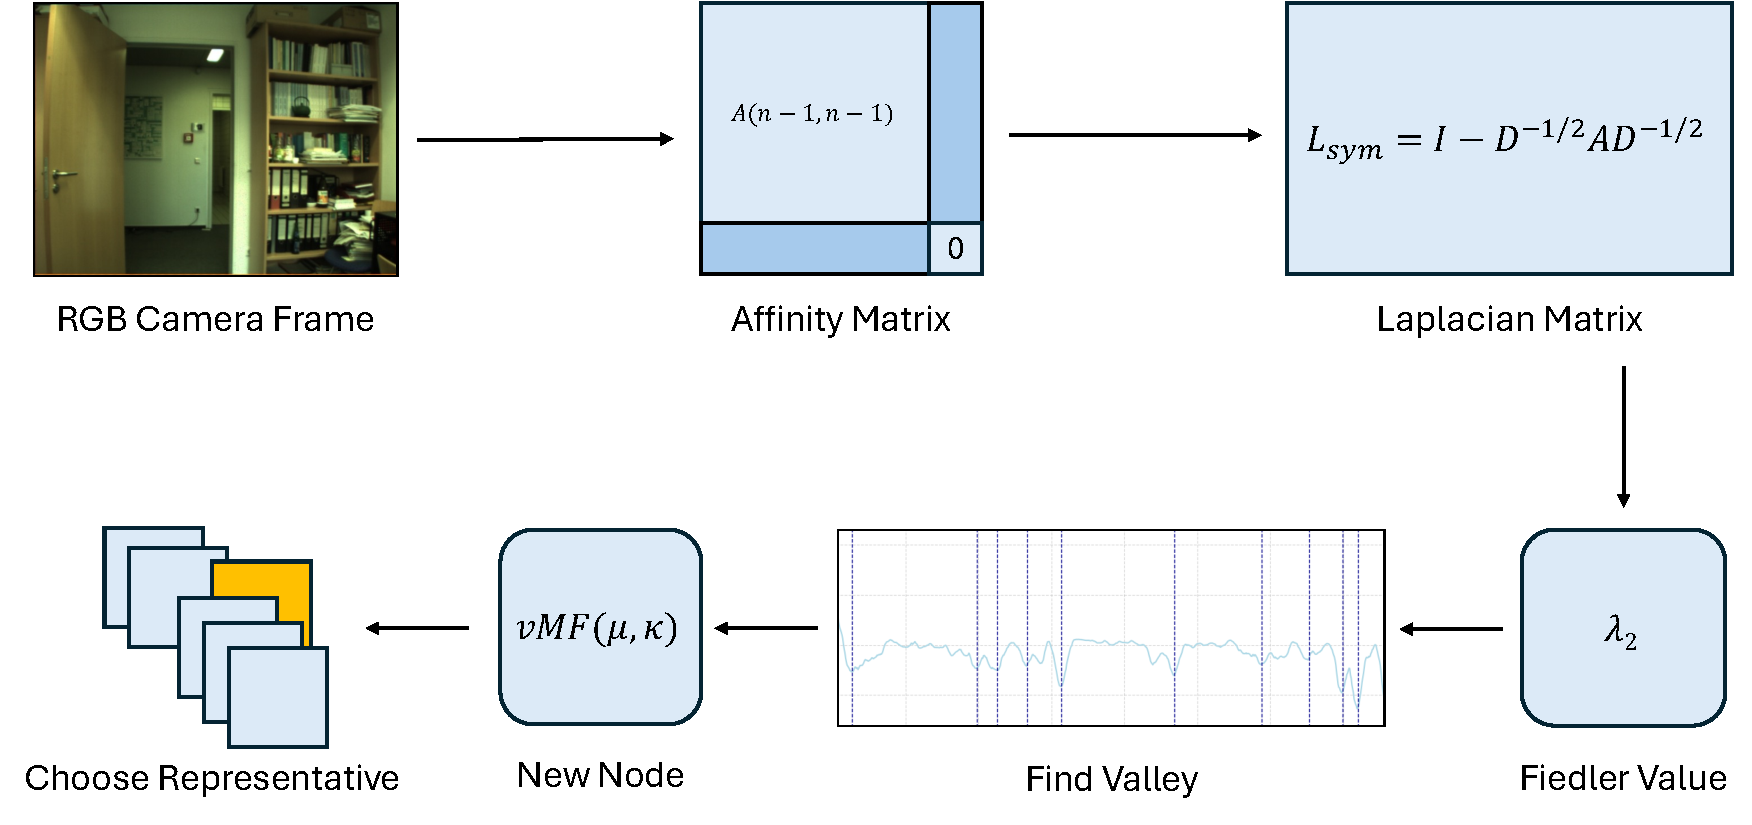
\includegraphics[width=\linewidth]{images/ac_pipeline.pdf}
    \caption{Online detection of node boundaries. Normalized descriptors from the current window create a weighted graph with non-negative cosine similarities. Its second Laplacian eigenvalue, $\lambda_2$, is high when the observations form one coherent group. A visual transition briefly divides the window into old and new appearances, producing a valley. The construction follows the algebraic-connectivity principle of~\cite{Boal2016}. \methodname adds non-negative affinities and an adaptive valley detector.}
    \label{fig:ac_pipeline}
\end{figure}

However, not every fluctuation should create a new place. To avoid this, the detector stores a possible minimum and accepts it only after the signal has risen far enough. Let $\Lambda_t$ contain the latest $h$ values of $\lambda_2$, let $m_t$ be their median, and let the median absolute deviation (MAD) be $\operatorname*{median}_{\lambda\in\Lambda_t}|\lambda-m_t|$. The required rise is
\begin{equation}
    \delta_t=\max\!\left(
    1.4826\,k_{\mathrm{valley}}
    \operatorname*{median}_{\lambda\in\Lambda_t}|\lambda-m_t|,
    \epsilon\right).
\end{equation}
The MAD measures recent variation while limiting the effect of isolated spikes~\cite{Rousseeuw1993}. The factor $1.4826$ scales it to match the standard deviation under Gaussian noise. The multiplier $k_{\mathrm{valley}}$ controls the required spike from a minimum, and the small floor $\epsilon$ keeps this requirement positive when the signal is flat.

Confirmation occurs after the transition because the detector must observe the rise. Nevertheless, the boundary is placed at the stored minimum, not at the later confirmation frame. Once a boundary is confirmed, the descriptors before it form a completed node.

\subsection{Node representation}
A node's descriptors may agree strongly or cover different views of the same place. To describe both their main direction and their spread, we fit a von Mises--Fisher (vMF) distribution on the unit hypersphere $S^{383}$~\cite{Mardia2000Directional}. This is a distribution over directions, concentrated around a unit mean vector:
\begin{equation}
    p(\mathbf{x}\mid\boldsymbol{\mu},\kappa)
    =C_d(\kappa)\exp\!\left(\kappa\boldsymbol{\mu}^{\top}\mathbf{x}\right),
\end{equation}
where the unit vector $\boldsymbol{\mu}$ gives the main appearance, the concentration $\kappa\geq0$ describes how tightly observations gather around it, and $C_d$ makes the density integrate to one. At $\kappa=0$ all directions are equally likely, while larger values indicate stronger agreement.

Figure~\ref{fig:vmf_sphere} shows these two parameters on an ordinary three-dimensional sphere. The mean direction represents where the distribution is centered, and concentration changes how far probability spreads around that direction. The same geometry carries over to the descriptor sphere $S^{383}$.

\begin{figure}[!htbp]
    \centering
    \begin{tikzpicture}[x=1cm,y=1cm,line cap=round,line join=round]
    \definecolor{vmfsphere}{RGB}{226,237,244}
    \definecolor{vmfedge}{RGB}{55,79,101}
    \definecolor{vmfgrid}{RGB}{126,151,169}
    \definecolor{vmfdensity}{RGB}{225,112,70}
    \definecolor{vmfsample}{RGB}{82,64,143}
    \definecolor{vmfmean}{RGB}{25,91,148}

    % Orthographic view. The unit mean direction is shared by both panels.
    \def\vmfRadius{1.48}
    \def\vmfMuX{0.28}
    \def\vmfMuY{0.18}
    \pgfmathsetmacro{\vmfMuZ}{sqrt(1-\vmfMuX*\vmfMuX-\vmfMuY*\vmfMuY)}
    \pgfmathsetmacro{\vmfMuScreen}{sqrt(\vmfMuX*\vmfMuX+\vmfMuY*\vmfMuY)}
    \pgfmathsetmacro{\vmfEllipseAngle}{atan2(\vmfMuY,\vmfMuX)+90}

    % An orthonormal basis of the tangent plane at mu.
    \pgfmathsetmacro{\vmfEoneX}{-\vmfMuY/\vmfMuScreen}
    \pgfmathsetmacro{\vmfEoneY}{ \vmfMuX/\vmfMuScreen}
    \pgfmathsetmacro{\vmfEtwoX}{-\vmfMuZ*\vmfMuX/\vmfMuScreen}
    \pgfmathsetmacro{\vmfEtwoY}{-\vmfMuZ*\vmfMuY/\vmfMuScreen}

    \newcommand{\drawVmfSphereBase}{%
        \shade[inner color=white,outer color=vmfsphere]
            (0,0) circle[radius=\vmfRadius];
    }

    % For q=p(x)/p(mu), mu^T x=1+ln(q)/kappa. Its orthographic
    % projection is the exact ellipse below. Every displayed cap remains
    % entirely on the visible hemisphere for this view.
    \newcommand{\drawVmfDensityBand}[3]{%
        \pgfmathsetmacro{\vmfLevel}{1+ln(#2)/(#1)}
        \pgfmathsetmacro{\vmfCapRadius}{\vmfRadius*sqrt(1-\vmfLevel*\vmfLevel)}
        \pgfmathsetmacro{\vmfCapMinor}{\vmfCapRadius*\vmfMuZ}
        \pgfmathsetmacro{\vmfCapX}{\vmfRadius*\vmfLevel*\vmfMuX}
        \pgfmathsetmacro{\vmfCapY}{\vmfRadius*\vmfLevel*\vmfMuY}
        \fill[vmfdensity!#3]
            (\vmfCapX,\vmfCapY)
            ellipse[x radius=\vmfCapRadius,
                    y radius=\vmfCapMinor,
                    rotate=\vmfEllipseAngle];
    }

    \newcommand{\drawVmfGrid}{%
        \draw[vmfgrid!42,line width=0.38pt]
            (-\vmfRadius,0)
            arc[start angle=180,end angle=360,
                x radius=\vmfRadius,y radius=0.35];
        \draw[vmfgrid!32,densely dashed,line width=0.38pt]
            (\vmfRadius,0)
            arc[start angle=0,end angle=180,
                x radius=\vmfRadius,y radius=0.35];
        \draw[vmfgrid!38,line width=0.38pt]
            (0,-\vmfRadius)
            arc[start angle=-90,end angle=90,
                x radius=0.46,y radius=\vmfRadius];
        \draw[vmfgrid!30,densely dashed,line width=0.38pt]
            (0,\vmfRadius)
            arc[start angle=90,end angle=270,
                x radius=0.46,y radius=\vmfRadius];
    }

    % A sample has polar cosine c and tangent-plane azimuth phi. Drawing the
    % opposite tangent direction as well makes the pair sum to 2c*mu.
    \newcommand{\drawVmfSamplePair}[2]{%
        \pgfmathsetmacro{\vmfSinTheta}{sqrt(1-(#1)*(#1))}
        \pgfmathsetmacro{\vmfTangentX}{cos(#2)*\vmfEoneX+sin(#2)*\vmfEtwoX}
        \pgfmathsetmacro{\vmfTangentY}{cos(#2)*\vmfEoneY+sin(#2)*\vmfEtwoY}
        \foreach \vmfSide in {-1,1}{
            \pgfmathsetmacro{\vmfPointX}{\vmfRadius*((#1)*\vmfMuX+\vmfSide*\vmfSinTheta*\vmfTangentX)}
            \pgfmathsetmacro{\vmfPointY}{\vmfRadius*((#1)*\vmfMuY+\vmfSide*\vmfSinTheta*\vmfTangentY)}
            \filldraw[fill=vmfsample,draw=white,line width=0.30pt]
                (\vmfPointX,\vmfPointY) circle[radius=0.025];
        }
    }

    \newcommand{\finishVmfSphere}{%
        \pgfmathsetmacro{\vmfMeanX}{\vmfRadius*\vmfMuX}
        \pgfmathsetmacro{\vmfMeanY}{\vmfRadius*\vmfMuY}
        \draw[-{Latex[length=1.9mm,width=1.25mm]},vmfmean,line width=1.25pt]
            (0,0)--(\vmfMeanX,\vmfMeanY);
        \draw[vmfedge,line width=0.85pt]
            (0,0) circle[radius=\vmfRadius];
    }

    % Broad fit. The ten polar cosines average to
    % coth(2)-1/2 = 0.5373147207275482. The varied azimuths avoid a ring.
    \begin{scope}[xshift=1.80cm]
        \drawVmfSphereBase
        \drawVmfDensityBand{2}{0.35}{13}
        \drawVmfDensityBand{2}{0.50}{22}
        \drawVmfDensityBand{2}{0.70}{36}
        \drawVmfDensityBand{2}{0.85}{58}
        \drawVmfGrid
        \foreach \vmfCos/\vmfAzimuth in {
            0.350000000000000/10,
            0.390000000000000/160,
            0.430000000000000/35,
            0.470000000000000/225,
            0.510000000000000/70,
            0.560000000000000/110,
            0.600000000000000/145,
            0.640000000000000/200,
            0.690000000000000/260,
            0.733147207275482/310}{
            \drawVmfSamplePair{\vmfCos}{\vmfAzimuth}
        }
        \finishVmfSphere
    \end{scope}

    % Concentrated fit. These ten polar cosines average to
    % coth(16)-1/16 = 0.9375000000000253.
    \begin{scope}[xshift=5.55cm]
        \drawVmfSphereBase
        \drawVmfDensityBand{16}{0.35}{13}
        \drawVmfDensityBand{16}{0.50}{22}
        \drawVmfDensityBand{16}{0.70}{36}
        \drawVmfDensityBand{16}{0.85}{58}
        \drawVmfGrid
        \foreach \vmfCos/\vmfAzimuth in {
            0.880000000000000/10,
            0.895000000000000/160,
            0.910000000000000/35,
            0.922000000000000/225,
            0.934000000000000/70,
            0.945000000000000/110,
            0.955000000000000/145,
            0.964000000000000/200,
            0.973000000000000/260,
            0.997000000000252/310}{
            \drawVmfSamplePair{\vmfCos}{\vmfAzimuth}
        }
        \finishVmfSphere
    \end{scope}
\end{tikzpicture}

    \caption{vMF distributions on $S^2$ with the same mean direction $\boldsymbol{\mu}$. Each sphere contains 20 unit observations, shown in purple. Warmer shading marks density levels at $35$, $50$, $70$ and $85\%$ of the peak. $\kappa=2$ (left) produces a broad distribution with $\bar r=0.54$, while $\kappa=16$ (right) produces a tight distribution with $\bar r=0.94$. The system follows the same principle on $S^{383}$.}
    \label{fig:vmf_sphere}
\end{figure}

\begin{figure*}[!t]
    \centering
    \begin{tikzpicture}[
    x=0.95cm,
    y=0.95cm,
    font=\footnotesize,
    >={Latex[length=2mm]},
    axis/.style={draw=black!18, line width=0.45pt},
    sphere/.style={draw=blue!30!black, line width=0.7pt},
    resultant/.style={-Latex, line width=1.25pt},
    captionlabel/.style={font=\footnotesize\bfseries, align=center},
    note/.style={font=\scriptsize, text=black!72, align=center},
    gate/.style={draw=orange!65!black, fill=orange!9, rounded corners=2pt,
        minimum width=3.2cm, minimum height=0.95cm, align=center},
    compare/.style={draw=violet!65!black, fill=violet!8, rounded corners=2pt,
        minimum width=4.15cm, minimum height=0.95cm, align=center}
]

% Every point below is placed with a polar coordinate at exactly the radius of
% its circle.  Each arrow ends at the arithmetic mean of those unit points:
% xbar = (1/m) sum_i x_i = rbar mu.
\node[note, text=black] at (4.35,5.15)
    {Dots: unit descriptors $\mathbf{x}_i\in S^{383}$};
\node[note, text=black] at (4.35,4.78)
    {Arrow: $\bar{\mathbf{x}}=\frac{1}{m}\sum_i\mathbf{x}_i=\bar r\,\boldsymbol{\mu}$;
     direction $=\boldsymbol{\mu}$, relative length $=\bar r$};

\coordinate (coherent) at (2.25,2.95);
\coordinate (variable) at (6.35,2.95);
\foreach \c in {coherent,variable}{
    \draw[sphere] (\c) circle (1.25);
    \draw[axis] ($(\c)+(-1.25,0)$) -- ($(\c)+(1.25,0)$);
    \draw[axis] ($(\c)+(0,-1.25)$) -- ($(\c)+(0,1.25)$);
}

% Coherent sample: angles 15 degrees +/- {0, 7, 14}; rbar = 0.985.
\pgfmathsetmacro{\coherentx}{(cos(1)+cos(8)+cos(15)+cos(22)+cos(29))/5}
\pgfmathsetmacro{\coherenty}{(sin(1)+sin(8)+sin(15)+sin(22)+sin(29))/5}
\foreach \a in {1,8,15,22,29}
    \fill[blue!67] ($(coherent)+(\a:1.25)$) circle (1.65pt);
\draw[resultant, blue!68!black] (coherent) --
    ($(coherent)+({1.25*\coherentx},{1.25*\coherenty})$);

% Dispersed sample: angles symmetric about 15 degrees; rbar = 0.394.
\pgfmathsetmacro{\variablex}{(cos(-90)+cos(-45)+cos(-5)+cos(35)+cos(75)+cos(120))/6}
\pgfmathsetmacro{\variabley}{(sin(-90)+sin(-45)+sin(-5)+sin(35)+sin(75)+sin(120))/6}
\foreach \a in {-90,-45,-5,35,75,120}
    \fill[orange!82] ($(variable)+(\a:1.25)$) circle (1.65pt);
\draw[resultant, orange!82!black] (variable) --
    ($(variable)+({1.25*\variablex},{1.25*\variabley})$);

\node[captionlabel] at (2.25,1.30) {Aligned views};
\node[note] at (2.25,0.93) {$\angle\boldsymbol{\mu}=15^\circ$ \quad $\bar r=0.985$};
\node[captionlabel] at (6.35,1.30) {Dispersed views};
\node[note] at (6.35,0.93) {$\angle\boldsymbol{\mu}=15^\circ$ \quad $\bar r=0.394$};
\node[gate] (maha) at (11.15,4.85) {\textbf{Mahalanobis gate}\\[-1pt]\scriptsize candidates A and B};
\node[compare] (overlap) at (15.65,4.85) {\textbf{vMF overlap (Eq.~\ref{eq:vmf-overlap})}\\[-1pt]
    \scriptsize $s_{ij}=\log\!\left(\int p_i p_j\,d\mathbf{x}\,/\,C_d(0)\right)$};
\draw[-Latex, line width=0.7pt, orange!75!black] (maha) -- (overlap);

\coordinate (candA) at (10.65,2.55);
\coordinate (query) at (13.75,2.55);
\coordinate (candB) at (16.85,2.55);
\foreach \c in {candA,query,candB}{
    \draw[sphere] (\c) circle (1.03);
    \draw[axis] ($(\c)+(-1.03,0)$) -- ($(\c)+(1.03,0)$);
    \draw[axis] ($(\c)+(0,-1.03)$) -- ($(\c)+(0,1.03)$);
}

% Candidate A: concentrated around 28 degrees; rbar = 0.989.
\pgfmathsetmacro{\candax}{(cos(16)+cos(22)+cos(28)+cos(34)+cos(40))/5}
\pgfmathsetmacro{\canday}{(sin(16)+sin(22)+sin(28)+sin(34)+sin(40))/5}
\foreach \a in {16,22,28,34,40}
    \fill[green!62!black] ($(candA)+(\a:1.03)$) circle (1.55pt);
\draw[resultant, green!62!black] (candA) --
    ($(candA)+({1.03*\candax},{1.03*\canday})$);

% Query: concentrated around 25 degrees; rbar = 0.989.
\pgfmathsetmacro{\queryx}{(cos(13)+cos(19)+cos(25)+cos(31)+cos(37))/5}
\pgfmathsetmacro{\queryy}{(sin(13)+sin(19)+sin(25)+sin(31)+sin(37))/5}
\foreach \a in {13,19,25,31,37}
    \fill[blue!67] ($(query)+(\a:1.03)$) circle (1.55pt);
\draw[resultant, blue!68!black] (query) --
    ($(query)+({1.03*\queryx},{1.03*\queryy})$);

% Candidate B: dispersed around -25 degrees; rbar = 0.446.
\pgfmathsetmacro{\candbx}{(cos(-125)+cos(-80)+cos(-45)+cos(-5)+cos(30)+cos(75))/6}
\pgfmathsetmacro{\candby}{(sin(-125)+sin(-80)+sin(-45)+sin(-5)+sin(30)+sin(75))/6}
\foreach \a in {-125,-80,-45,-5,30,75}
    \fill[red!66] ($(candB)+(\a:1.03)$) circle (1.55pt);
\draw[resultant, orange!82!black] (candB) --
    ($(candB)+({1.03*\candbx},{1.03*\candby})$);

\draw[-Latex, line width=1pt, green!60!black] (13.75,3.82) --
    node[above, note, text=green!48!black] {strong overlap} (10.65,3.82);
\draw[-Latex, line width=1pt, red!65!black] (13.75,3.82) --
    node[above, note, text=red!58!black] {weak overlap} (16.85,3.82);

\node[captionlabel] at (10.65,1.08) {Candidate A};
\node[note] at (10.65,0.72) {$\angle\boldsymbol{\mu}_A=28^\circ$};
\node[note] at (10.65,0.42) {$\bar r_A=0.989$};
\node[captionlabel] at (13.75,1.08) {Query node};
\node[note] at (13.75,0.72) {$\angle\boldsymbol{\mu}_q=25^\circ$};
\node[note] at (13.75,0.42) {$\bar r_q=0.989$};
\node[captionlabel] at (16.85,1.08) {Candidate B};
\node[note] at (16.85,0.72) {$\angle\boldsymbol{\mu}_B=-25^\circ$};
\node[note] at (16.85,0.42) {$\bar r_B=0.446$};
\end{tikzpicture}

    \caption{Directional node representation. Dots are unit descriptors and arrows are sample means $\bar{\mathbf{x}}=\bar r\boldsymbol{\mu}$. Left: aligned and dispersed views can have the same mean direction but different resultant lengths. Right: Candidate A matches the query more closely in direction and spread than Candidate B, giving stronger vMF overlap. The system applies the same principle on $S^{383}$.}
    \label{fig:vmf_model}
\end{figure*}

For a segment of $m$ descriptors $\mathbf{x}_i$, the resultant vector and its normalized length are
\begin{equation}
    \mathbf{r}=\sum_{i=1}^{m}\mathbf{x}_i, \qquad
    \bar r=\frac{\lVert\mathbf{r}\rVert}{m}.
\end{equation}
The vector $\mathbf{r}$ points toward the average appearance, so $\boldsymbol{\mu}=\mathbf{r}/\lVert\mathbf{r}\rVert$. Its normalized length $\bar r\in[0,1]$ approaches one when the frames agree and falls as they spread. The concentration $\kappa$ is estimated using the high-dimensional approximation of Banerjee~\etalcite{Banerjee2005vMF}
\begin{equation}
    \kappa \simeq \frac{\bar r(d-\bar r^2)}{1-\bar r^2}, \qquad d=384.
\end{equation}
Therefore, a high $\kappa$ indicates a visually consistent node and a low value indicates greater variation among its observations. A single frame cannot reveal a spread, so nodes with just one frame are assigned $\kappa=0$.

Two nodes are compared by the overlap of their fitted distributions. Unlike the cosine similarity between two representatives, this score uses both their main directions and their concentrations. For nodes $i$ and $j$, the log overlap relative to a uniform distribution is
\begin{equation}    
\label{eq:vmf-overlap}
\begin{split}
    s_{ij}={}&\log C_d(\kappa_i)+\log C_d(\kappa_j)-\log C_d(0)\\
    &-\log C_d\!\left(\left\lVert\kappa_i\boldsymbol{\mu}_i+
    \kappa_j\boldsymbol{\mu}_j\right\rVert\right).
\end{split}
\end{equation}
The combined vector grows when two concentrated distributions point in the same direction and shrinks when they disagree. A diffuse node with $\kappa\approx0$ contributes little evidence either way. Subtracting $\log C_d(0)$ makes an uninformative uniform model the zero reference: positive scores mean more agreement than that reference and negative scores mean less. The calculation is performed with logarithms because the normalizing constants become extremely large or small in 384 dimensions.

Figure~\ref{fig:vmf_model} illustrates how the same mean direction can arise from either aligned or dispersed observations, and how both direction and spread affect candidate comparison.

\subsection{Loop closure and graph construction}
\label{sec:loop-closure}
Every node except the first is linked to its predecessor, extending the recorded route with a sequential edge. It may also receive a loop edge if the robot has returned to an already visited place. The two most recent nodes are excluded from this search because sequential edges already describe their local relation. Revisit search starts when at least five eligible historical nodes exist.

For a new node $i$ and an older node $j$, let $\mathbf{e}_{ij}\in\mathbb{R}^2$ be the difference between their odometric positions. Under the hypothesis that both nodes represent the same place, the expected displacement is zero. The observed displacement should therefore be small relative to the uncertainty accumulated between the observations. We use
\begin{equation}
    S_{ij}=(B_i-B_j)_{xy}+\sigma_{\mathrm{place}}^2I+10^{-6}I.
\end{equation}
Here $\sigma_{\mathrm{place}}=\qty{0.5}{\metre}$, and the budget difference comes from Equation~\ref{eq:motion-budget}. The additional place term allows a nonzero separation between representative frames of the same local region, even when little motion uncertainty has accumulated. It is a fixed modeling choice, not an estimated sensor error. The final term provides numerical regularization, and all terms in $S_{ij}$ are in square metres. The squared Mahalanobis distance measures displacement relative to this budget~\cite{Mahalanobis1936}:
\begin{equation}
    d^2_{ij}=\mathbf{e}_{ij}^{\top}S_{ij}^{-1}\mathbf{e}_{ij}.
\end{equation}
A candidate passes when $d^2_{ij}\leq5.991$, which is the nominal $95\%$ boundary for a two-dimensional Gaussian. The same displacement can therefore be rejected after a short motion but allowed after a longer, more uncertain one. Passing candidates are ranked by $d^2_{ij}+\log\det S_{ij}$, twice the Gaussian negative log-likelihood up to a constant. The first term rewards a small displacement relative to uncertainty, while the second penalizes a broad budget that might present every node as plausible.

Figure~\ref{fig:mahalanobis_search} illustrates the position gate. The implemented XY budget is isotropic, so each candidate has a circular acceptance region. Its radius grows with the uncertainty accumulated since that candidate was observed.

\begin{figure}[!htbp]
    \centering
    \begin{tikzpicture}[x=1cm,y=1cm,line cap=round,line join=round,font=\scriptsize]
    \definecolor{gateblue}{RGB}{57,106,177}
    \definecolor{acceptgreen}{RGB}{34,139,74}
    \definecolor{rejectred}{RGB}{204,54,54}

    % One illustrative isotropic budget; actual candidates can have different s.
    \fill[gateblue!10] (0,0) circle[radius=1.65];
    \draw[gateblue,very thick] (0,0) circle[radius=1.65];
    \coordinate (query) at (0,0);
    \coordinate (acceptedOne) at (0.90,0.65);
    \coordinate (acceptedTwo) at (-1.05,0.35);
    \coordinate (rejected) at (1.78,1.05);
    \draw[black!30,densely dotted] (query)--(acceptedOne);
    \draw[black!30,densely dotted] (query)--(acceptedTwo);
    \draw[black!30,densely dotted] (query)--(rejected);
    \draw[-{Latex[length=1.5mm]},gateblue] (query)--(0,-1.65)
        node[midway,right,text=gateblue] {$\sqrt{5.991}\,s$};
    \fill[black!82] (query) ++(0,0.13)--++(0.13,-0.13)--++(-0.13,-0.13)--++(-0.13,0.13)--cycle;
    \filldraw[fill=acceptgreen,draw=white,line width=0.8pt] (acceptedOne) circle[radius=0.115];
    \filldraw[fill=acceptgreen,draw=white,line width=0.8pt] (acceptedTwo) circle[radius=0.115];
    \filldraw[fill=rejectred,draw=white,line width=0.8pt] (rejected) circle[radius=0.125];
    \draw[white,line width=0.85pt] ($(rejected)+(-0.055,-0.055)$)--($(rejected)+(0.055,0.055)$);
    \draw[white,line width=0.85pt] ($(rejected)+(-0.055,0.055)$)--($(rejected)+(0.055,-0.055)$);
\end{tikzpicture}

    \caption{Position gating with an isotropic uncertainty budget $S=s^2I$. The diamond marks zero displacement. For the illustrated budget, candidates inside the circle satisfy $\lVert\mathbf{e}\rVert\leq\sqrt{5.991}\,s$: green candidates pass and the red candidate fails. In an actual search, $s$ can differ between historical nodes because their accumulated budgets differ. The threshold is the nominal $95\%$ Gaussian boundary in two dimensions.}
    \label{fig:mahalanobis_search}
\end{figure}

If no candidates are found, the graph receives only its sequential edge. A single compatible candidate is accepted without visual validation. This policy assumes that spatial isolation is sufficient evidence for association, so it can fail when the uncertainty budget admits the wrong place. Visual comparison is reserved for the ambiguous case with several candidates. Let $q_k$ be the new node and $h_j$ one candidate. The query and up to two recent nodes are aligned with the stored sequence on either side of $h_j$. For direction $\sigma\in\{-1,+1\}$ and $1\leq M_{\sigma}\leq3$ available pairs, the mean score is
\begin{equation}
    S_{\sigma}(q_k,h_j)=\frac{1}{M_{\sigma}}
    \sum_{r=0}^{M_{\sigma}-1}
    s_{\mathrm{vMF}}(q_{k-r},h_{j+\sigma r}).
\end{equation}
Here $s_{\mathrm{vMF}}$ is the node overlap from Equation~\ref{eq:vmf-overlap}, and $M_{\sigma}$ is the number of available pairs. Only sequential edges define the context (earlier loop edges are not followed). This allows matching in either direction of travel. For instance, a stored sequence room--door--corridor can thus match a revisit observed as corridor--door--room. The larger of the two directional scores is kept.

For the ambiguous case, let $H$ contain all eligible historical nodes, let $\mathcal{C}\subseteq H$ contain those passing the geometric gate, and let $s_j=\max_{\sigma}S_{\sigma}(q_k,h_j)$. The candidates in $\mathcal{C}$ are tested in increasing order of $d^2_{ij}+\log\det S_{ij}$. Let $\mathcal{W}_j=\{h\in H\setminus\mathcal{C}:s_h\leq s_j\}$ contain excluded nodes with weaker or equal visual scores. We form the comparison pool as
\begin{equation}
\begin{aligned}
    \mathcal{P}_j &=
    \begin{cases}
        \mathcal{C}, & |\mathcal{C}|\geq5,\\
        \mathcal{C}\cup\mathcal{W}_j, & |\mathcal{C}|<5,
    \end{cases}\\
    \mathcal{O}_j &= \{s_h:h\in\mathcal{P}_j,\ h\neq j\}.
\end{aligned}
\end{equation}
The scores in $\mathcal{O}_j$ retain one entry per node, including equal values. Thus the candidate is compared with every other geometrically compatible node. When there are fewer than five compatible nodes, weaker or equal scores from outside the gate also provide background evidence. Stronger excluded matches are omitted so that a place already rejected by geometry cannot veto an association solely through its appearance. This is a heuristic choice that relies on the geometric gate being appropriate.

Let $m_j$ be the median of $\mathcal{O}_j$ and $a_j$ its MAD. Candidate $j$ passes when
\begin{equation}
    s_j>m_j+1.4826\,k_{\mathrm{visual}}a_j.
\end{equation}
In words, its visual sequence must stand above the typical competing score by a margin set by the spread of those scores. The candidate's own score is excluded from this calculation, and strict inequality rejects ties when the MAD is zero. The first candidate to pass receives a loop edge. If none passes, only the sequential edge remains.

\subsection{Text-to-node retrieval experiment}
After mapping, each node retains at most three views: the segment's first frame, last frame and the frame closest to its mean appearance (most representative). We present a potential application of the proposed system in which users can send natural language queries to the robot for node retrieval (subsequent navigation is outside the scope of this work).

Given a text request such as ``take me to the kitchen,'' CLIP embeds the target phrase and retained node views in a shared space~\cite{radford2021learningtransferablevisualmodels}. Generic command openings are removed, and the target phrase is inserted into four photographic prompt templates. Their embeddings are averaged into one text representation and each node is scored by its highest cosine similarity with the text across its retained views. A softmax using CLIP's learned scale converts these similarities into relative scores.

A difference below $0.1$ between the two highest softmax scores marks a request as unresolved, and a singleton map is also treated as indeterminate. This exploratory rule measures separation between suggestions, not whether the destination exists. The interface presents ranked suggestions and publishes a navigation destination only after the user explicitly confirms a candidate from the current query.

\section{Results}

We evaluate node creation, loop association and map geometry, then compare visual descriptors and loop closure variants. Runtime and storage are reported afterwards, followed by the text-to-node retrieval experiment. Table~\ref{tab:metrics} defines the reported metrics.

\begin{table*}[t]
\centering
\caption{Metric notation used throughout the results. The suffix $@r$ denotes evaluation at spatial tolerance $r$ in metres.}

\label{tab:metrics}
\footnotesize
\setlength{\tabcolsep}{5pt}
\begin{tabular}{>{\raggedright\arraybackslash}p{0.18\textwidth}p{0.61\textwidth}>{\raggedright\arraybackslash}p{0.15\textwidth}}
\hline
Notation & Definition & Unit \\
\hline
$N_{\mathrm{nodes}}$, $N_{\mathrm{loops}}$ & Numbers of graph nodes and accepted loop edges. & $[-]$ \\
$\rho_{\mathrm{node}}$ & Mean node creation rate across sequences. & [nodes/1000 frames] \\
$\mathrm{CV}_{\mathrm{node}}$ & Coefficient of variation of the node creation rate across sequences. $[0,\infty)$. & $[-]$ \\
$R_{\mathrm{trans}}$, Purity & Room-transition recall and frame-weighted node purity. $[0,1]$. & $[-]$ \\
Seg./episode & Mean node segments per semantic episode. & [segments/episode] \\
TP, FP, FN & True-positive, false-positive, and false-negative loop closures. & $[-]$ \\
$P$, $R$, $F_1@r$ & Loop closure precision, recall, and their harmonic mean at spatial tolerance $r$. $[0,1]$. & $[-]$ \\
$C_{\mathrm{map}}@r$ & Fraction of the ground truth trajectory within $r$ of a node. $[0,1]$. & $[-]$ \\
$R@k$, MRR & Retrieval recall at rank $k$ and mean reciprocal rank for present destinations. $[0,1]$. & $[-]$ \\
$C_{\mathrm{ret}}$, $A_{\mathrm{ans}}$, $R_{\mathrm{rej}}$ & Selected-present fraction, accuracy of those selections, and unresolved rate for absent destinations. $[0,1]$. & $[-]$ \\
\hline
\end{tabular}
\end{table*}

\subsection{Dataset}
The evaluation uses four sequences from the CoSy Localization Database (COLD)~\cite{COLD} and three from the Complex Indoor Dataset with Semantic Information and Multi-Sensor Data (CID-SIMS)~\cite{Zhang2023CIDSIMS}, comprising $13{,}196$ processed frames. The selected Freiburg and Saarbr\"ucken traversals, from COLD, contain repeated offices, corridors and room transitions under changing illumination. The apartment traversals, from CID-SIMS, provide a second visual domain with furnished domestic spaces and accurate reference trajectories. Recorded wheel odometry is supplied to every mapping configuration. Ground truth poses and semantic annotations are used for evaluation, never in online node-boundary or loop-association decisions.

\subsection{Experimental setup and parameters}
All experiments ran on an Apple MacBook Pro M3 inside an Ubuntu~24.04 development container with Robot Operating System~2 (ROS~2) Jazzy, Python~3.12 and PyTorch~2.13.0. The container exposed neither a CUDA device nor Apple's Metal acceleration, so inference ran on the CPU. Therefore, the reported times describe this setup and are not GPU benchmarks. Mapping uses the \texttt{dinov2\_vits14}~\cite{oquab2024dinov2learningrobustvisual} checkpoint and text retrieval uses \texttt{clip-vit-base-patch32}.

COLD images were sampled at approximately \qty{5}{\hertz} in dataset time. CID-SIMS was recorded at \qty{30}{\hertz}, so every sixth image was selected, yielding the same effective sampling rate. The parameter set shown in Table~\ref{tab:parameters} was kept across all seven traversals, except when an experiment explicitly replaced the detector or descriptor backend.

\begin{table}[t]
\centering
\caption{Mapping parameters, held fixed except in the stated component comparisons. The $\alpha$ units are defined in Equation~\ref{eq:motion-budget}.}
\label{tab:parameters}
\small
\begin{tabular}{ll}
\hline
Parameter & Value \\
\hline
Visual window $n$ & 30 frames ($\sim\qty{6}{\second}$) \\
Valley multiplier $k_{\mathrm{valley}}$ & 2.0 \\
Robust history $h$ & 300 samples ($\sim\qty{60}{\second}$) \\
Detector warm-up & 30 samples \\
Visual multiplier $k_{\mathrm{visual}}$ & 2.0 \\
Squared geometric threshold & 5.991 \\
Place scale $\sigma_{\mathrm{place}}$ & \qty{0.5}{\metre} \\
Sequence context & Up to 3 pairs per direction \\
$(\alpha_1,\alpha_2)$ & $(0.025,0.005)$ \\
$(\alpha_3,\alpha_4)$ & $(0.010,0.0025)$ \\
\hline
\end{tabular}
\end{table}

\subsection{Evaluation protocol}
All compared methods receive the same images and odometry. They also share the node detector and the parameters in Table~\ref{tab:parameters}, except when the experiment explicitly replaces one component. We score loop closure at distances $r\in\{0.5,1,2,3\}$~m because a topological node represents a local region, not an exact point. At a given $r$, a revisit opportunity exists when the ground truth position of a new node lies within $r$~m of an eligible earlier node. The two most recent nodes are excluded because sequential edges already represent their local relation. Opportunities are counted per new-node query rather than per nearby pair. An accepted edge is a true positive (TP) if its endpoints satisfy this rule and a false positive (FP) otherwise. A query with an available revisit that is not correctly associated contributes a false negative (FN), so an incorrect accepted edge may contribute both an FP and an FN. We compute precision, recall and $F_1$ as
\begin{equation}
\begin{aligned}
    P &= \frac{\mathrm{TP}}{\mathrm{TP}+\mathrm{FP}}, \qquad
    R = \frac{\mathrm{TP}}{\mathrm{TP}+\mathrm{FN}}, \\
    F_1 &= 2\frac{PR}{P+R}
           = \frac{2\mathrm{TP}}{2\mathrm{TP}+\mathrm{FP}+\mathrm{FN}}.
\end{aligned}
\end{equation}
If a denominator is zero, the corresponding score is set to zero. These counts use loop edges only, as including the guaranteed sequential edges would hide poor revisit detection behind many automatic connections. Aggregate scores pool TP, FP and FN across sequences before computing the ratios. A correct association here means that representative-frame positions satisfy the spatial tolerance, not necessarily that they form a traversable edge.

We also report trajectory coverage by representative nodes and node-position root-mean-square error (RMSE) after a best-fit planar rigid alignment. Coverage measures spatial sampling, while aligned RMSE measures the remaining node-position error.

\subsection{Node-creation sensitivity}
\begin{table*}[t]
\centering
\caption{Node creation sensitivity and comparison with a fixed-prominence detector. $N_{\mathrm{nodes}}$, $\rho_{\mathrm{node}}$ and $\mathrm{CV}_{\mathrm{node}}$ use all seven sequences. The remaining metrics are averaged over the four annotated COLD traversals. The fixed prominence is calibrated on Freiburg A and then transferred unchanged.}
\label{tab:node_sensitivity}
\footnotesize
\setlength{\tabcolsep}{5pt}
\begin{tabular}{lrrrrrr}
\hline
Detector & \begin{tabular}[c]{@{}c@{}}$N_{\mathrm{nodes}}$\end{tabular} & \begin{tabular}[c]{@{}c@{}}$\rho_{\mathrm{node}}$\end{tabular} & \begin{tabular}[c]{@{}c@{}}$\mathrm{CV}_{\mathrm{node}}$\end{tabular} & \begin{tabular}[c]{@{}c@{}}$R_{\mathrm{trans}}$\end{tabular} & \begin{tabular}[c]{@{}c@{}}Purity\end{tabular} & \begin{tabular}[c]{@{}c@{}}Seg./episode\end{tabular}\\
\hline
Adaptive, $k=1.0$ & 217 & 16.943 & 0.134 & \textbf{0.643} & \textbf{0.908} & 3.508\\
Adaptive, $k=1.5$ & 183 & 14.265 & 0.134 & 0.580 & 0.895 & 3.267\\
Adaptive, $k=2.0$ (final) & 149 & 11.464 & 0.138 & 0.467 & 0.859 & 2.943\\
Adaptive, $k=2.5$ & 119 & 9.057 & \textbf{0.103} & 0.417 & 0.826 & 2.534\\
Adaptive, $k=3.0$ &  99 & 7.318 & 0.160 & 0.368 & 0.765 & 2.253\\
Fixed, $\delta=0.130$ & 158 & 12.341 & 0.235 & 0.596 & 0.896 & 3.099\\
\hline
\end{tabular}
\end{table*}

Figure~\ref{fig:lambda2_run} illustrates the node extraction process from Section~\ref{sec:node-extraction} over a complete laboratory traversal. Algebraic connectivity remains high while the descriptors in the window form one cohesive group and falls when two appearances coexist, producing varied valley depths. The detector evaluates the recovery from each minimum against recent signal variation, rather than requiring the same recovery everywhere. It identifies $29$ valleys and therefore creates $30$ nodes, including the initial segment before the first boundary.

\begin{figure}[!htbp]
    \centering
    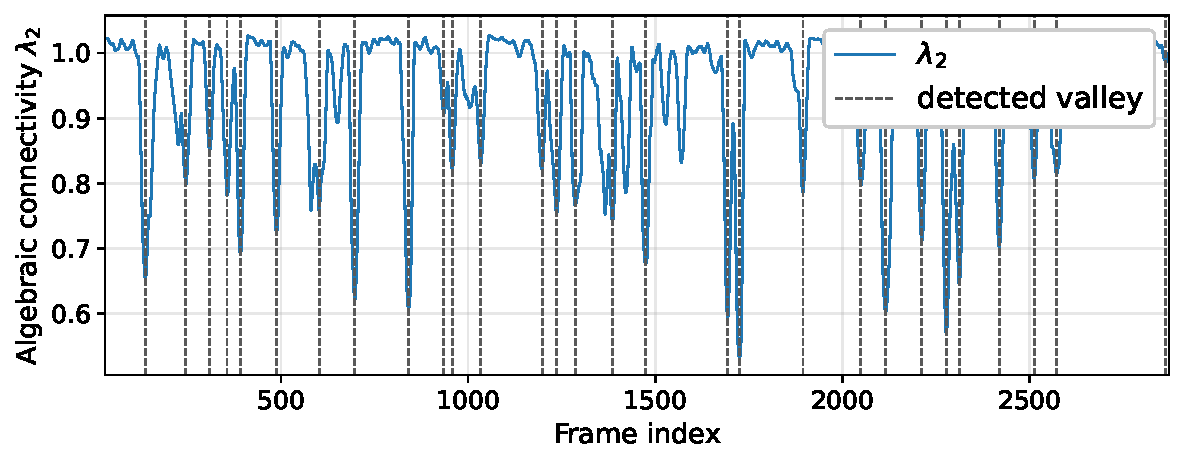
\includegraphics[width=\linewidth]{images/lambda2_freiburg_a.pdf}
    \caption{Node extraction over the complete Freiburg A traversal. The blue signal is the algebraic connectivity $\lambda_2$ of the sliding visual graph and dashed vertical lines denote minima confirmed by the adaptive median-and-MAD hysteresis rule. Valleys occur when two weakly connected appearances temporarily share the window.}
    \label{fig:lambda2_run}
\end{figure}

The multiplier $k_{\mathrm{valley}}$ controls the prominence required to accept a boundary. Lower values retain smaller valleys and create more, shorter nodes, while larger values produce a more compact graph but may join visually different parts of the trajectory. We test $k_{\mathrm{valley}}\in\{1,1.5,2,2.5,3\}$. The adaptive rule is also compared with the same hysteresis detector using a fixed prominence $\delta=0.130$, calibrated to reproduce the $30$ nodes of $k=2$ on Freiburg A and then transferred unchanged to every other sequence.

Table~\ref{tab:node_sensitivity} reports the total number of nodes, the mean rate per $1000$ frames and its coefficient of variation (CV) across sequences. Lower $\mathrm{CV}_{\mathrm{node}}$ indicates more consistent node creation rates per frame. It does not alone imply better segmentation, since scene structure and travel speed can require different rates. On the four annotated COLD traversals, transition recall measures the fraction of room changes assigned one-to-one to a boundary within $15$ frames (\qty{3}{\second}), using the matching that maximizes the number of detected transitions. Purity is the frame-weighted proportion of each node assigned to its dominant room. The segments-per-episode metric reveals when those scores improve simply because a continuous room visit has been divided repeatedly. These semantic metrics are averaged across the four sequences. Labels are used only for this diagnostic.

As expected, increasing $k$ trades detail for compactness. Adaptive $k=1$ creates $217$ nodes and gives the highest transition recall and purity, but divides each semantic episode into $3.508$ segments on average. At $k=3$, the graph contains only $99$ nodes, with fewer divisions per episode but lower transition recall and purity. Therefore, there is no setting that maximizes semantic agreement and compactness simultaneously.

The same trade-off appears in loop closure. Adaptive $k=1$ gives the highest aggregate $F_1$ at \qty{0.5}{\metre} and, by a margin of $0.001$, at \qty{3}{\metre}; $k=1.5$ leads at \qty{1}{\metre}, while $k=2$ gives the highest value at \qty{2}{\metre}. We retain $k_{\mathrm{valley}}=2$ as a common operating point because it reduces the graph from $217$ to $149$ nodes, performs best at the \qty{2}{\metre} tolerance and avoids the lower purity and loop closure performance observed for $k\geq2.5$. This choice is supported by the same seven-sequence study reported here. The four tolerances are retained throughout to show how the result changes with the definition of a revisit.

After calibration on Freiburg A, the fixed detector gives a node-rate CV of $0.235$ across sequences, compared with $0.138$ for adaptive $k=2$. The fixed rule has higher transition recall and purity, while the adaptive rule uses fewer nodes overall and gives higher loop closure precision, recall and $F_1$ at every evaluated radius, with an $F_1$ advantage ranging from $0.045$ to $0.230$. The adaptive setting therefore offers a useful compromise in this study: more consistent node creation rates and better loop association, but lower agreement with the room annotations.

\subsection{Topological mapping}
Table~\ref{tab:loops} scores the same completed graphs at each evaluation distance. They contain $149$ nodes and $27$ accepted loop edges. A stricter radius classifies more edges as incorrect spatial associations. Increasing the radius admits broader place correspondence but also creates additional revisit opportunities, so recall does not need to increase. At \qty{2}{\metre}, $25$ accepted edges are true positives, giving precision $0.926$, recall $0.521$ and $F_1=0.667$.

\begin{table*}[t]
\centering
\caption{Loop closure results of the complete vMF gate. $N_{\mathrm{nodes}}$ and $N_{\mathrm{loops}}$ give the size of each completed graph and the number of accepted edges. The remaining columns report $F_1$ after applying each spatial tolerance to the same graph.}
\label{tab:loops}
\small
\begin{tabular}{llrrrrrr}
\hline
Dataset & Sequence & $N_{\mathrm{nodes}}$ & $N_{\mathrm{loops}}$ & $F_1@0.5\,\mathrm{m}$ & $F_1@1\,\mathrm{m}$ & $F_1@2\,\mathrm{m}$ & $F_1@3\,\mathrm{m}$\\
\hline
\multirow{4}{*}{COLD} & Freiburg A       & 30 & 3 & 0.400 & 0.333 & 0.200 & 0.125\\
 & Freiburg Extended& 22 & 3 & 0.800 & 0.571 & 0.600 & 0.500\\
 & Saarbr\"ucken A  & 32 & 3 & 0.000 & 0.286 & 0.500 & 0.375\\
 & Saarbr\"ucken Extended & 16 & 2 & 0.000 & 0.667 & 1.000 & 0.500\\
\hline
\multirow{3}{*}{CID-SIMS} & Apartment 1      & 18 & 8 & 0.364 & 0.308 & 0.941 & 0.800\\
 & Apartment 2      & 11 & 2 & 0.000 & 0.667 & 0.571 & 0.500\\
 & Apartment 3      & 20 & 6 & 0.000 & 0.000 & 0.800 & 0.632\\
\hline
All & Aggregate        & 149 & 27 & 0.286 & 0.320 & 0.667 & 0.505\\
\hline
\end{tabular}
\end{table*}

Figures~\ref{fig:cold_maps} and~\ref{fig:cid_maps} show the resulting connectivity, with nodes placed at ground-truth representative-frame coordinates for visualization. Freiburg A has one true and two false accepted loops at \qty{2}{\metre}; the other three COLD traversals contain only true accepted loops at this tolerance. All sixteen accepted apartment loops also satisfy the \qty{2}{\metre} criterion. These counts describe accepted associations, while Table~\ref{tab:loops} also reflects the revisits that were missed.

\begin{table*}[t]
\centering
\caption{Geometric quality of the final maps. $C_{\mathrm{map}}@r$ is the fraction of the ground truth trajectory lying within radius $r$ of a node. $\mathrm{RMSE}$ measures node-position error after one best-fit planar rigid alignment and therefore retains odometric drift.}
\label{tab:mapquality}
\small
\setlength{\tabcolsep}{3.5pt}
\begin{tabular}{llrrrrr}
\hline
Dataset & Sequence & $C_{\mathrm{map}}@0.5\,\mathrm{m}$ & $C_{\mathrm{map}}@1\,\mathrm{m}$ & $C_{\mathrm{map}}@2\,\mathrm{m}$ & $C_{\mathrm{map}}@3\,\mathrm{m}$ & $\mathrm{RMSE}$ [m]\\
\hline
\multirow{4}{*}{COLD} & Freiburg A         & 0.492 & 0.771 & 0.977 & 1.000 & 3.792\\
 & Freiburg Ext.      & 0.647 & 0.893 & 0.969 & 1.000 & 1.886\\
 & Saarbr\"ucken A   & 0.453 & 0.685 & 0.911 & 0.998 & 4.179\\
 & Saarbr\"ucken Ext.& 0.545 & 0.808 & 0.999 & 1.000 & 1.039\\
\hline
\multirow{3}{*}{CID-SIMS} & Apartment 1        & 0.630 & 0.894 & 1.000 & 1.000 & 0.439\\
 & Apartment 2        & 0.409 & 0.623 & 0.930 & 0.994 & 0.365\\
 & Apartment 3        & 0.707 & 0.914 & 1.000 & 1.000 & 0.502\\
\hline
\end{tabular}
\end{table*}

\begin{figure*}[p]
    \centering
    \begin{subfigure}[t]{0.47\textwidth}
        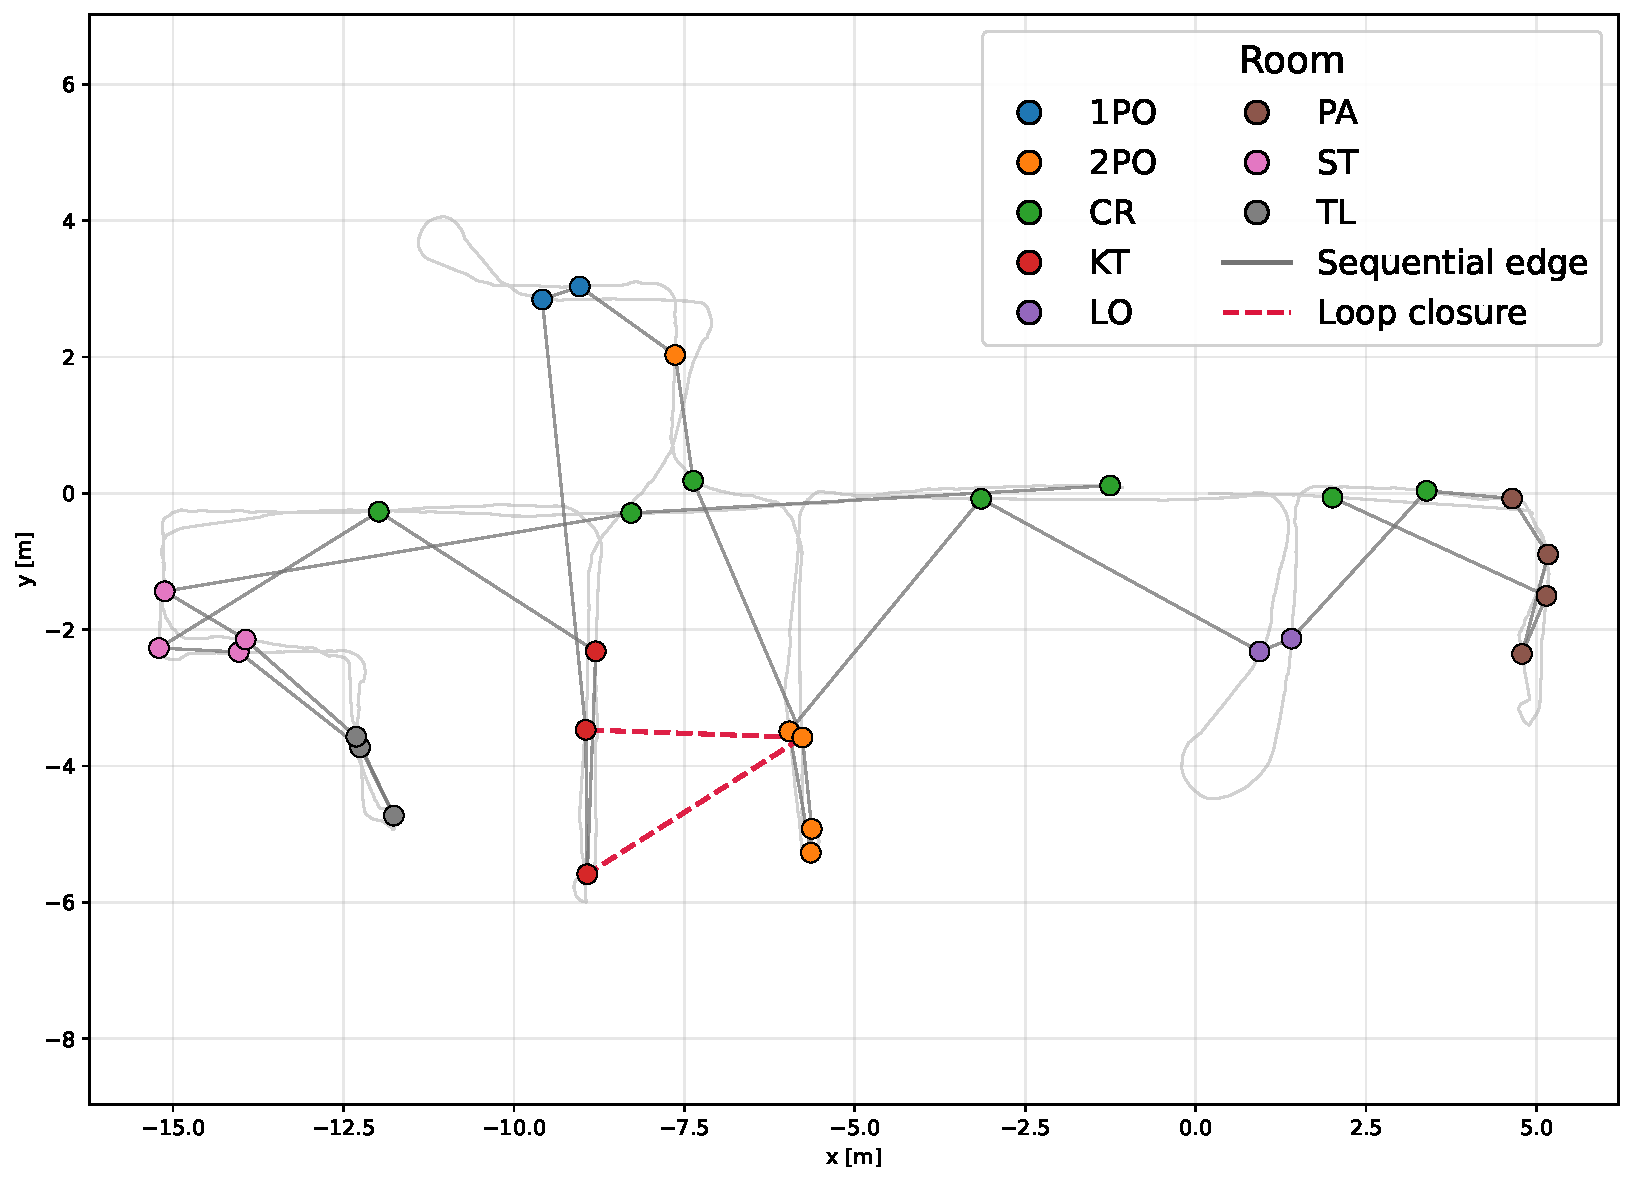
\includegraphics[width=\linewidth]{images/map_freiburg_a.pdf}
        \caption{Freiburg A.}
    \end{subfigure}\hfill
    \begin{subfigure}[t]{0.47\textwidth}
        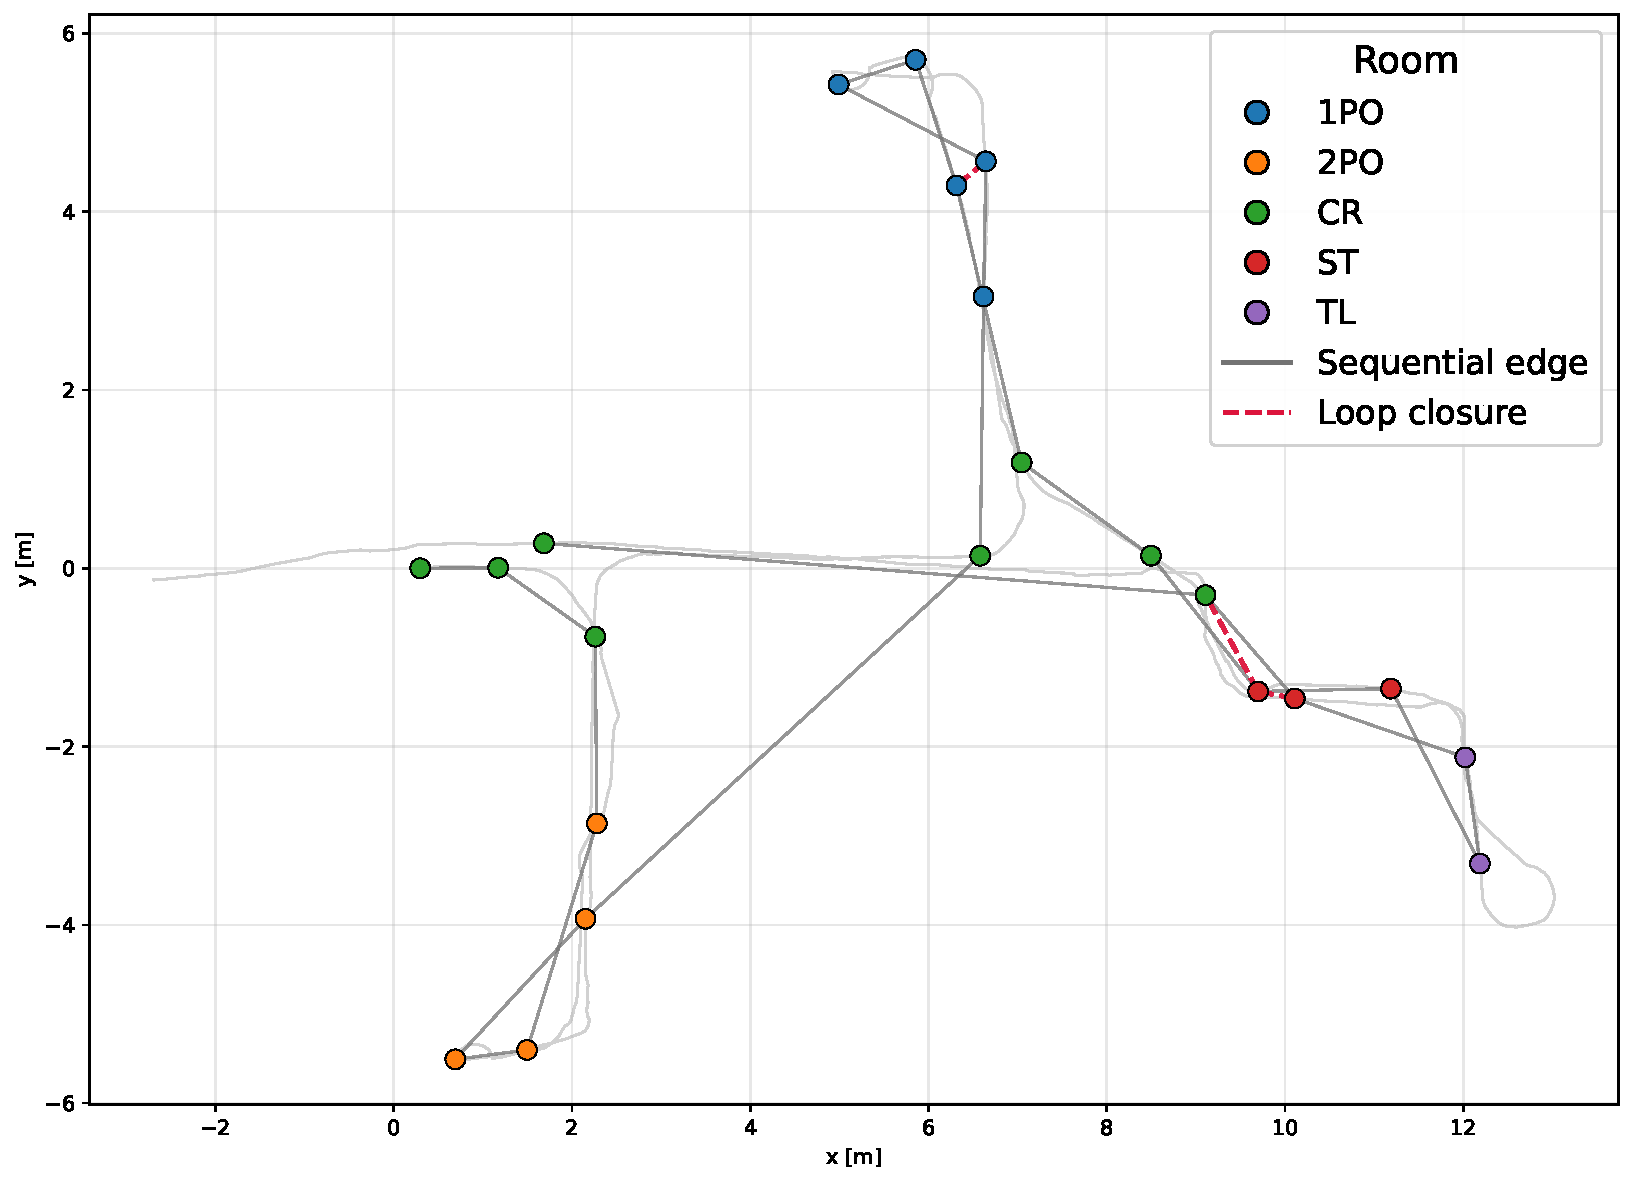
\includegraphics[width=\linewidth]{images/map_freiburg_extended.pdf}
        \caption{Freiburg Extended.}
    \end{subfigure}

    \begin{subfigure}[t]{0.47\textwidth}
        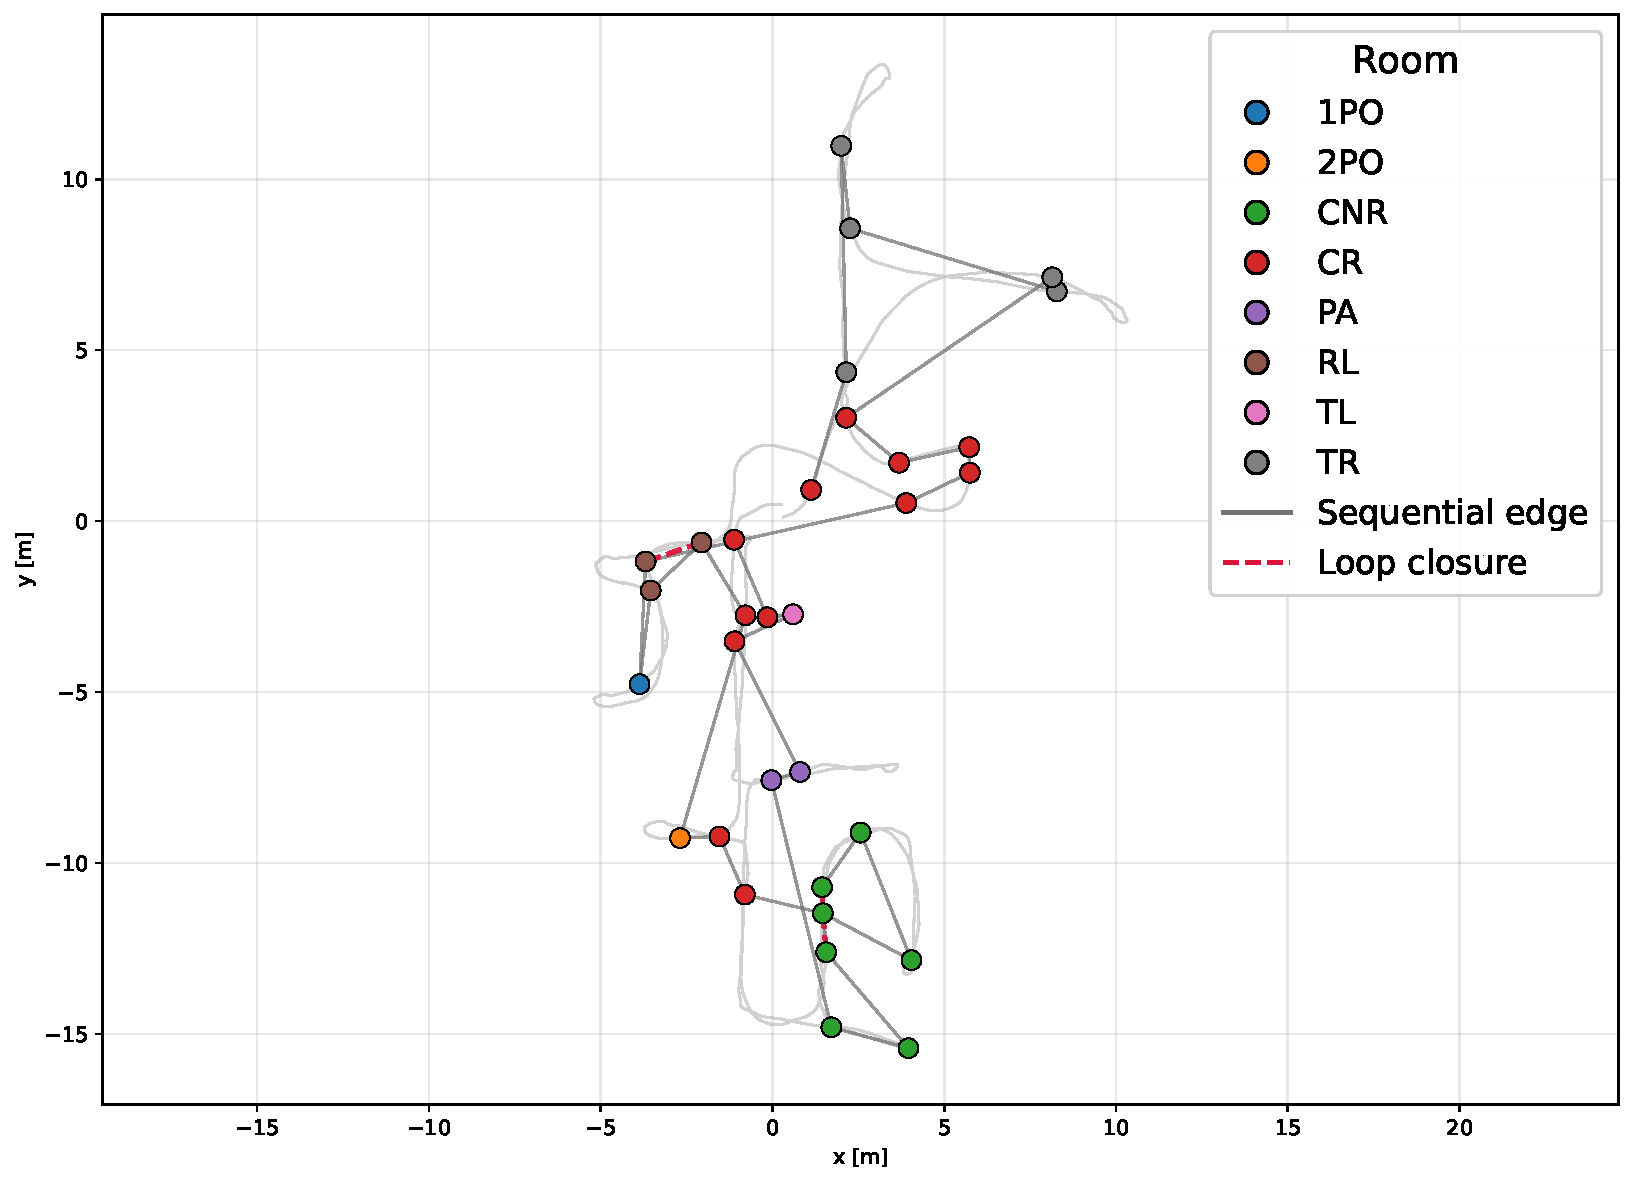
\includegraphics[width=\linewidth]{images/map_saarbruecken_a.pdf}
        \caption{Saarbr\"ucken A.}
    \end{subfigure}\hfill
    \begin{subfigure}[t]{0.47\textwidth}
        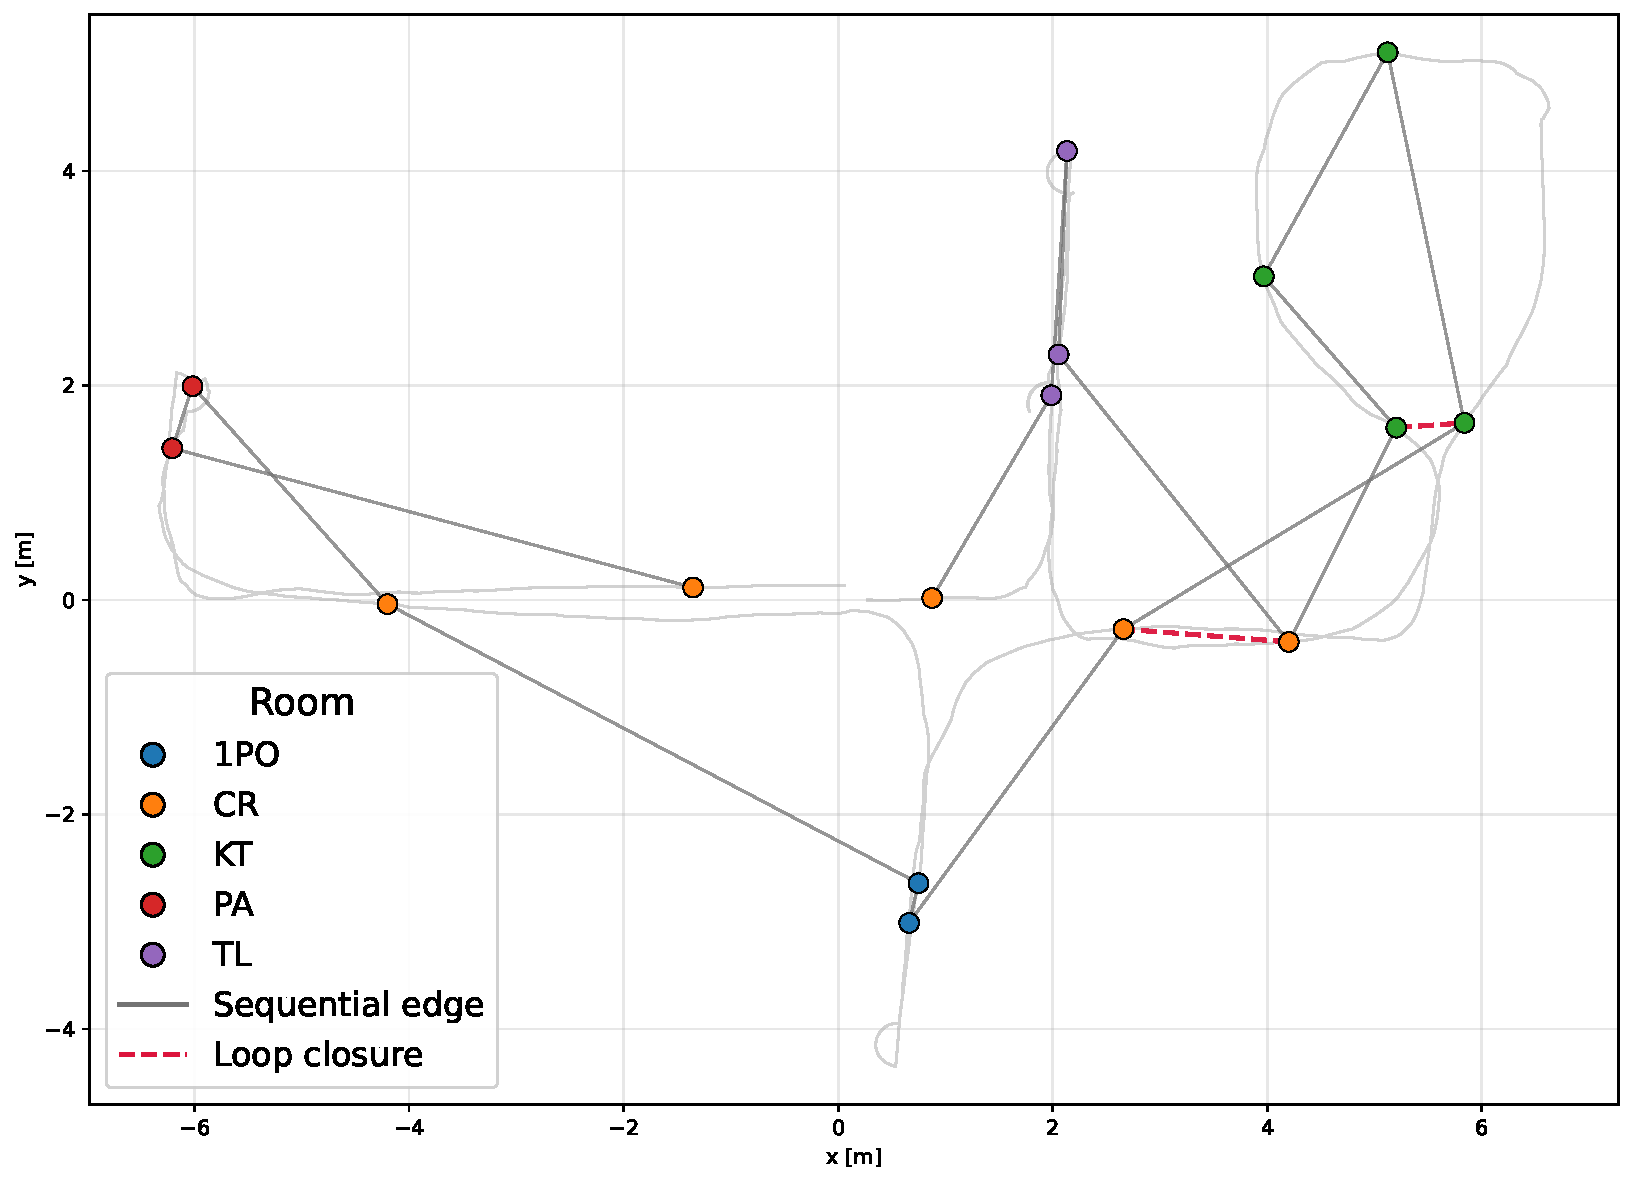
\includegraphics[width=\linewidth]{images/map_saarbruecken_extended.pdf}
        \caption{Saarbr\"ucken Extended.}
    \end{subfigure}

    \caption{Topological connectivity for the four COLD traversals, plotted at ground-truth representative-frame positions. The light curve provides the ground truth trajectory for spatial context, solid gray edges connect consecutive observations and dashed red edges are accepted loop closures. Node colors show the available room annotations: one-person office (1PO), two-person office (2PO), corridor (CR), conference room (CNR), kitchen (KT), large office (LO), printer area (PA), robotics laboratory (RL), stairs (ST), toilet (TL) and terminal room (TR).}
    \label{fig:cold_maps}
\end{figure*}

\begin{figure*}[p]
    \centering
    \begin{subfigure}[t]{0.30\textwidth}
        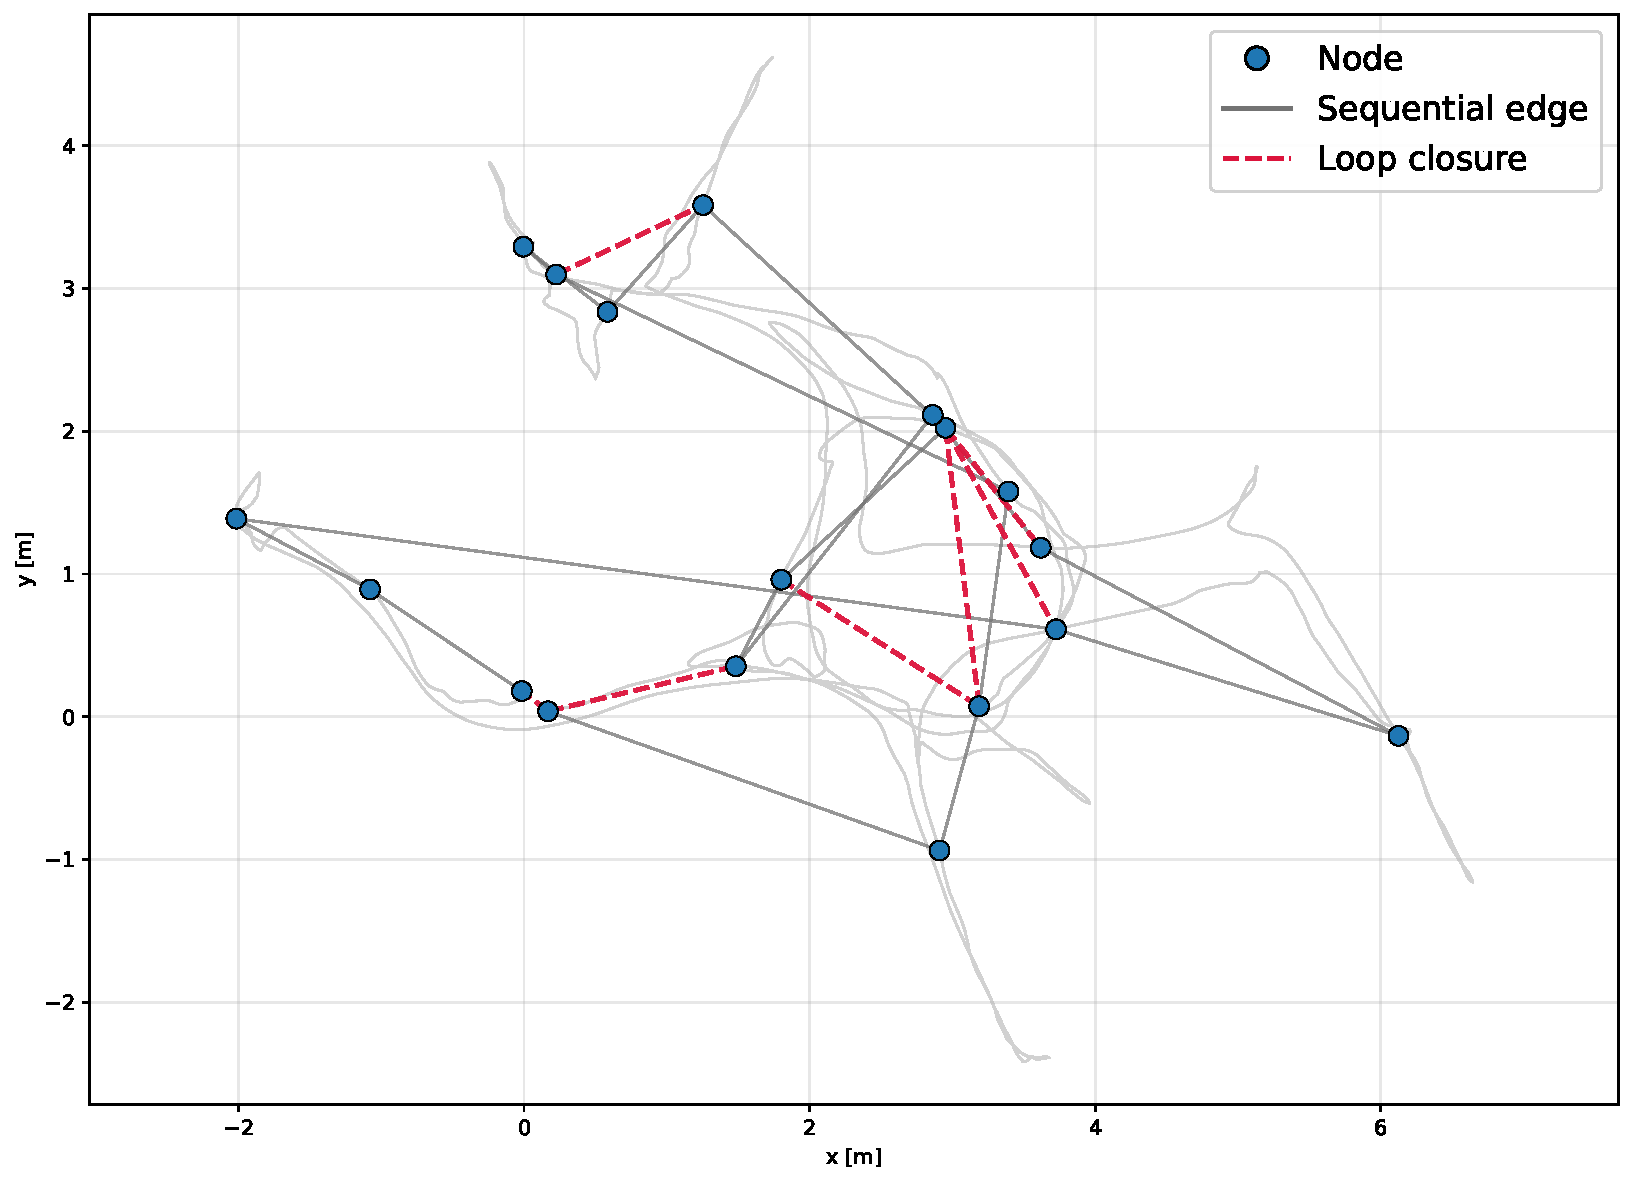
\includegraphics[width=\linewidth]{images/map_apartment_1.pdf}
        \caption{Apartment 1.}
    \end{subfigure}\hfill
    \begin{subfigure}[t]{0.30\textwidth}
        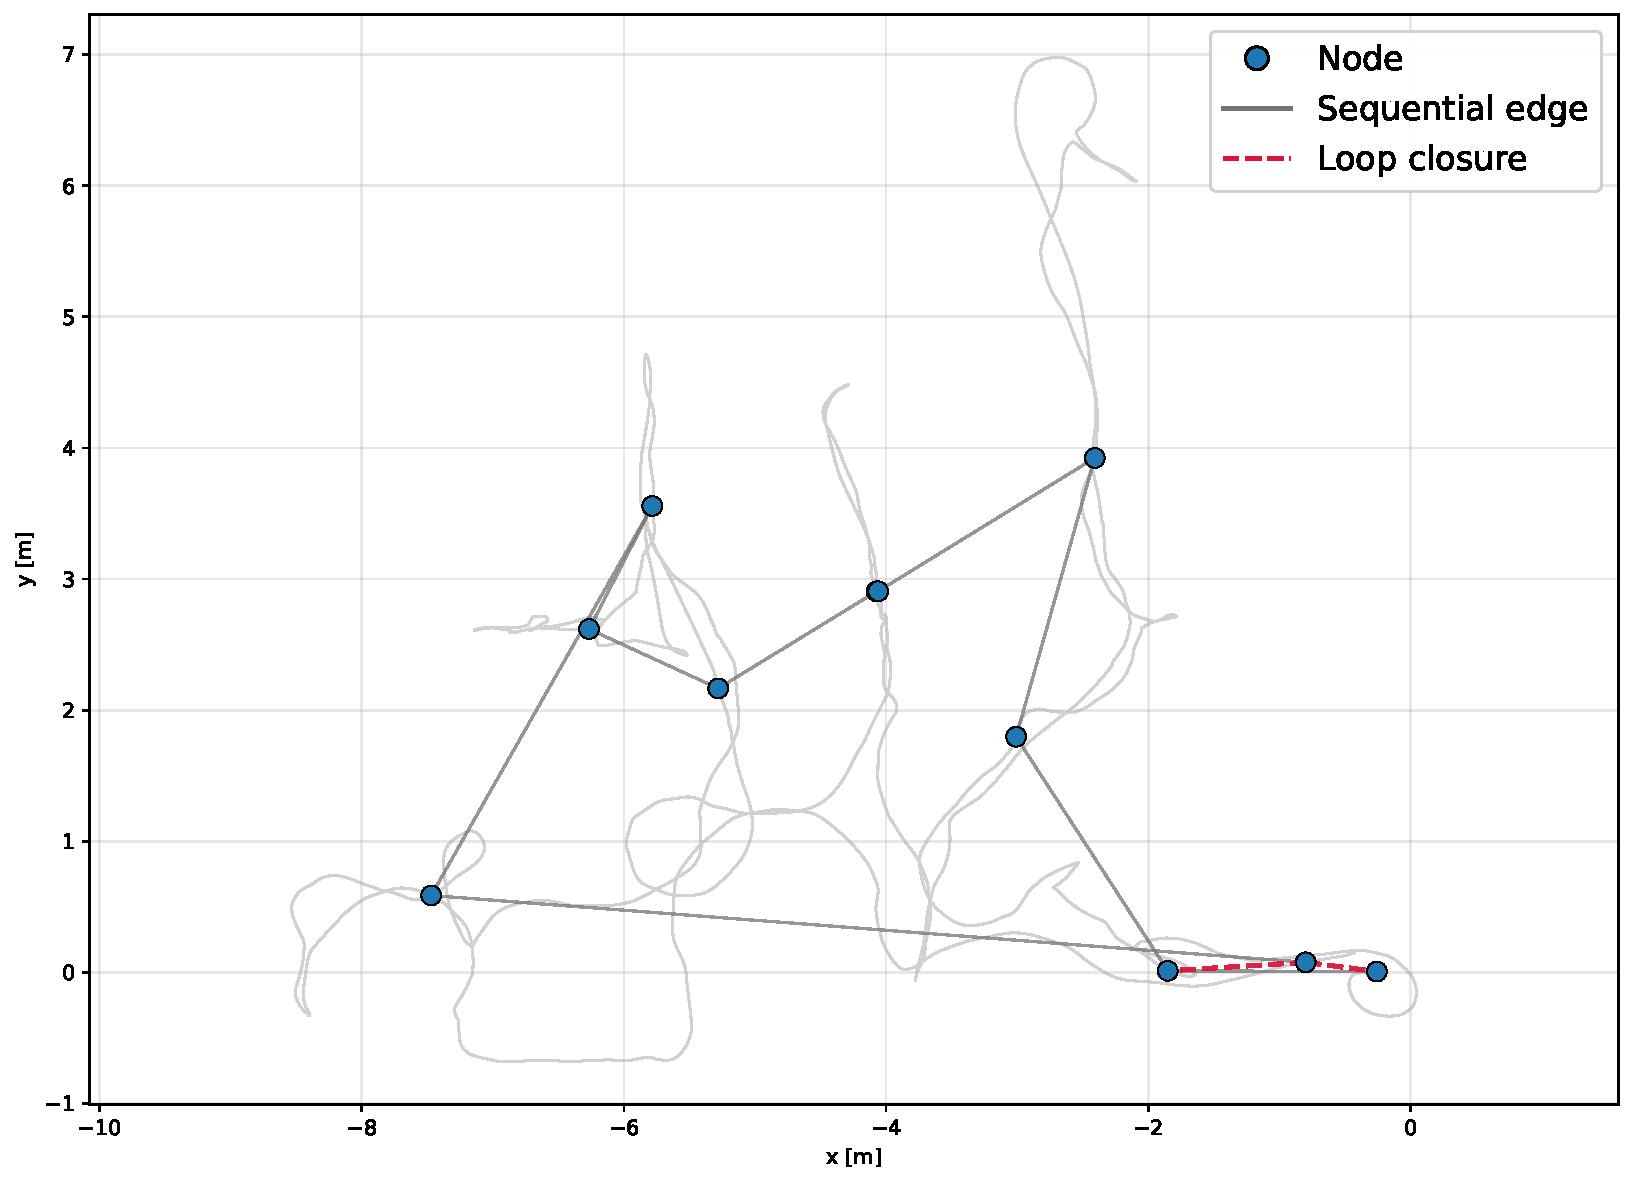
\includegraphics[width=\linewidth]{images/map_apartment_2.pdf}
        \caption{Apartment 2.}
    \end{subfigure}\hfill
    \begin{subfigure}[t]{0.30\textwidth}
        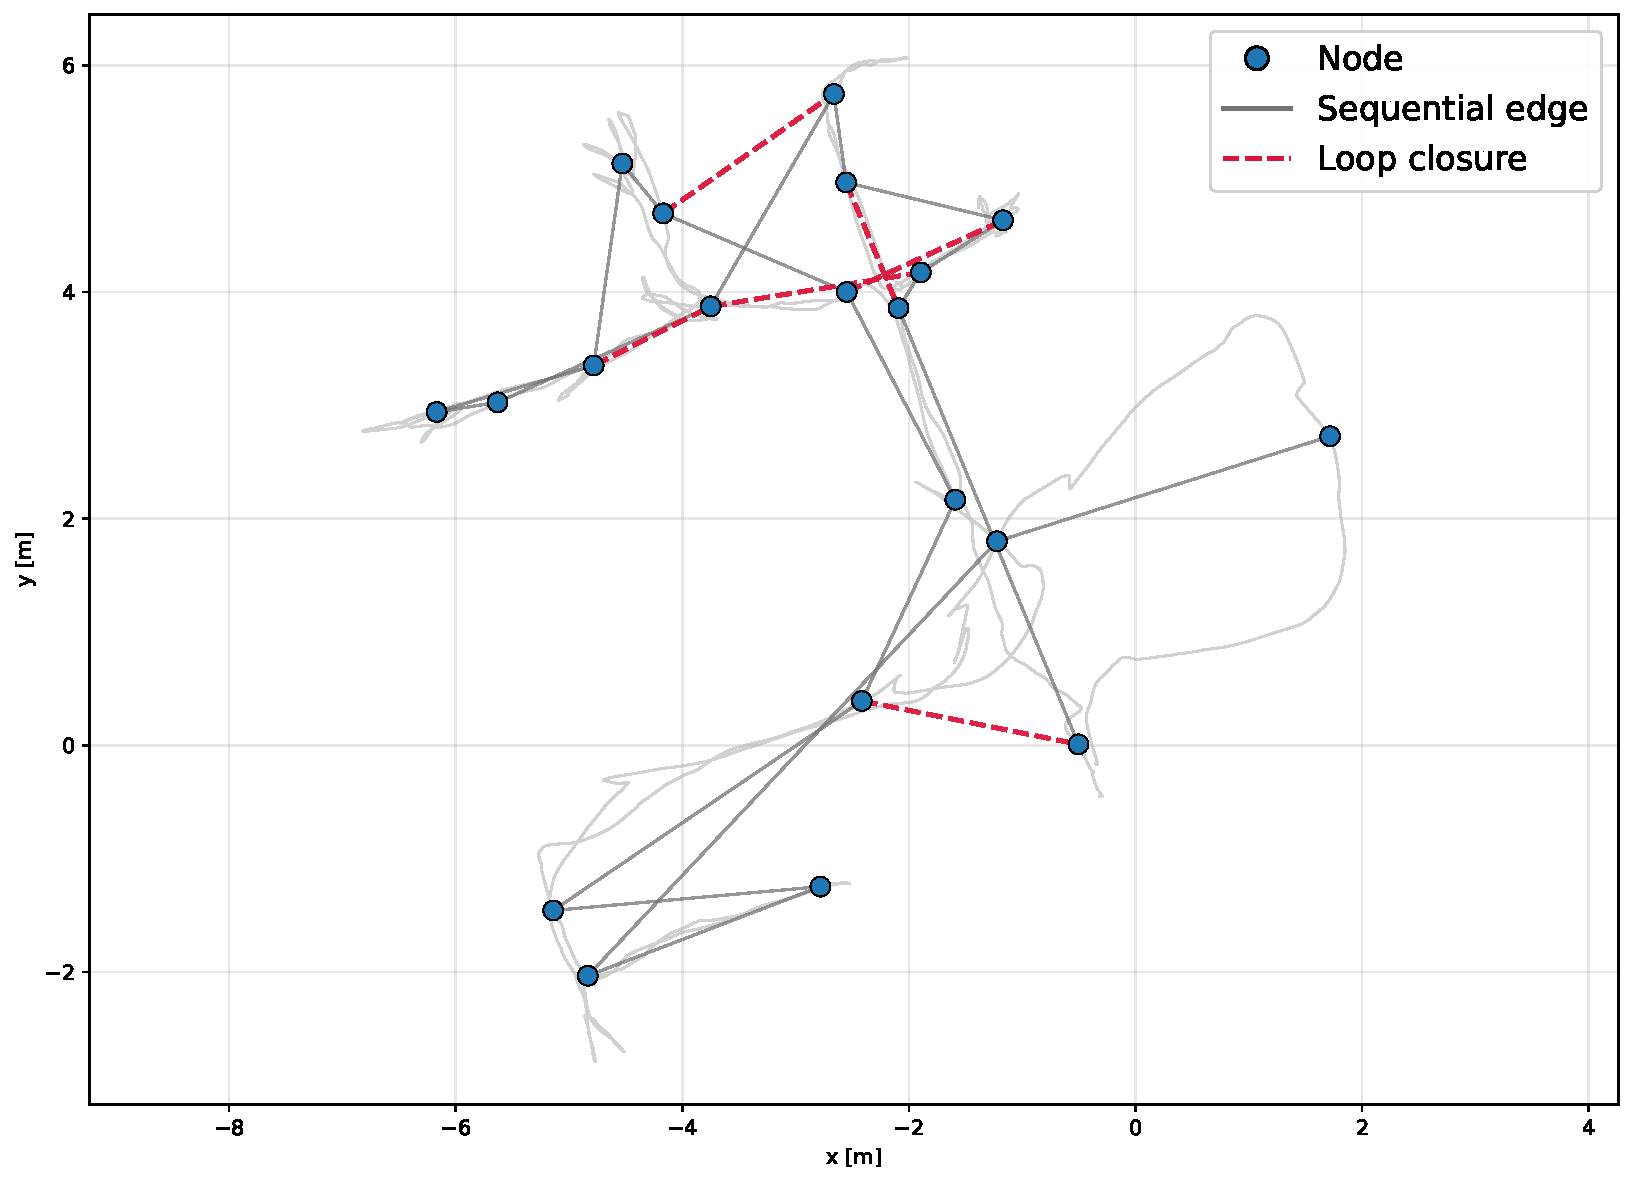
\includegraphics[width=\linewidth]{images/map_apartment_3.pdf}
        \caption{Apartment 3.}
    \end{subfigure}
    \caption{Topological connectivity for the three CID-SIMS traversals, plotted at ground-truth representative-frame positions. Solid gray edges connect consecutive observations and dashed red edges are accepted loop closures. CID-SIMS does not provide the room annotations used in Fig.~\ref{fig:cold_maps}, so node colors carry no semantic meaning.}
    \label{fig:cid_maps}
\end{figure*}

Table~\ref{tab:mapquality} reports geometric quality. Coverage at \qty{0.5}{\metre} ranges from $0.409$ to $0.707$, and every traversal reaches at least $0.994$ at \qty{3}{\metre}. Apartment node-position RMSE stays below \qty{0.51}{\metre}, while COLD errors range from \qtyrange{1.04}{4.18}{\metre} after rigid alignment. The system retains recorded odometry without global correction, so these maps still carry substantial position error.

\subsection{Visual representation and retrieval baseline}
This comparison asks whether a descriptor designed for visual place retrieval also produces a better topology inside the loop closure architecture of Section~\ref{sec:loop-closure}. AnyLoc builds a global image descriptor from the local patch features of a Vision Transformer. Our controlled adaptation reads the value-projection features from the final transformer block and combines them with signed generalized-mean (GeM) pooling at $p=3$. In practical terms, strong and repeated feature responses receive more weight while their sign is preserved. The resulting vector replaces the standard DINOv2~\cite{oquab2024dinov2learningrobustvisual} descriptor throughout the same mapper. Images, odometry and the node-detector settings are shared.

Published AnyLoc uses the much larger ViT-G/14 backbone. To keep the representation and compute budget controlled, both methods use the same ViT-S/14 backbone on the available CPU. The comparison therefore isolates final-block patch features and GeM pooling under the same resources.

Table~\ref{tab:baseline} compares $F_1$ in the laboratory and apartment domains at every evaluation radius. The aggregate ordering depends on the radius: \methodname performs better at \qty{0.5}{\metre} and \qty{2}{\metre}, whereas the AnyLoc adaptation performs better at \qty{1}{\metre} and \qty{3}{\metre}. The domain breakdown adds further context. \methodname leads on COLD through \qty{2}{\metre} and on CID-SIMS at \qty{2}{\metre}, while AnyLoc leads on the remaining domain--radius combinations. The comparison concerns the complete mapper because changing the descriptors can also change the node boundaries and available revisit opportunities.

\begin{table*}[t]
\centering
\caption{Loop closure $F_1$ comparison with the AnyLoc-inspired baseline across spatial tolerances and visual domains. Both methods receive the same image stream and odometry and use the same ViT-S/14 backbone.}
\label{tab:baseline}
\small
\setlength{\tabcolsep}{3.5pt}
\begin{tabular}{rcccccc}
\hline
& \multicolumn{2}{c}{COLD} & \multicolumn{2}{c}{CID-SIMS} & \multicolumn{2}{c}{All}\\
Tolerance [m] & \methodname & Adaptation & \methodname & Adaptation & \methodname & Adaptation\\
\hline
0.5 & \textbf{0.400} & 0.133 & 0.200 & \textbf{0.320} & \textbf{0.286} & 0.250\\
1.0 & \textbf{0.435} & 0.261 & 0.222 & \textbf{0.562} & 0.320 & \textbf{0.436}\\
2.0 & \textbf{0.500} & 0.276 & \textbf{0.821} & 0.773 & \textbf{0.667} & 0.575\\
3.0 & 0.346 & \textbf{0.400} & 0.681 & \textbf{0.731} & 0.505 & \textbf{0.587}\\
\hline
\end{tabular}
\end{table*}

Table~\ref{tab:tolerance_baseline} separates precision and recall. At \qty{0.5}{\metre}, recall is equal and \methodname has higher precision. At \qty{1}{\metre}, the AnyLoc adaptation improves both measures. At the two larger distances, \methodname has higher precision, but at \qty{3}{\metre} its lower recall gives the adaptation a higher $F_1$. Because descriptors also change node boundaries, the methods do not face identical revisit opportunities: at \qty{2}{\metre}, there are 48 for \methodname and 41 for the adaptation.

\begin{table}[!htbp]
    \centering
    \caption{Aggregate loop closure sensitivity to spatial tolerance. Both completed graphs are rescored at every radius.}
    \label{tab:tolerance_baseline}
    \small
    \setlength{\tabcolsep}{3pt}
    \begin{tabular}{rcccccc}
    \hline
    & \multicolumn{3}{c}{\methodname} & \multicolumn{3}{c}{AnyLoc-inspired}\\
    Tolerance [m] & $P$ & $R$ & $F_1$ & $P$ & $R$ & $F_1$\\
    \hline
    0.5 & \textbf{0.185} & \textbf{0.625} & \textbf{0.286} & 0.156 & \textbf{0.625} & 0.250\\
    1.0 & 0.296 & 0.348 & 0.320 & \textbf{0.375} & \textbf{0.522} & \textbf{0.436}\\
    2.0 & \textbf{0.926} & \textbf{0.521} & \textbf{0.667} & 0.656 & 0.512 & 0.575\\
    3.0 & \textbf{0.926} & 0.347 & 0.505 & 0.844 & \textbf{0.450} & \textbf{0.587}\\
    \hline
    \end{tabular}
\end{table}

\subsection{Loop closure ablation}
This ablation study tests the sources of evidence in the loop closure system described in Section~\ref{sec:loop-closure}. The complete method uses the odometry-based position gate followed, when necessary, by vMF verification. The cosine variant preserves the same candidates and decision structure but replaces distribution overlap with the symmetric multi-view score: for each retained view, take its largest cosine similarity with the other node's views, then average those maxima in both directions. Geometry-only accepts compatible candidates without appearance verification. Visual-only keeps the selected vMF sequence evidence and removes geometric restriction altogether, while the fixed-threshold variant accepts cosine similarity above $0.7$. Every other mapping component is unchanged, so the comparison only concerns the loop closure detection mechanism.

Table~\ref{tab:ablation} reveals two effects of different magnitude. The essential improvement comes from restricting visual reasoning with geometry. Removing that restriction produces $57$ false closures for the adaptive visual-only variant, while a fixed threshold still produces $28$. Repeated appearance alone is not a safe basis for graph connectivity. Geometry-only achieves the highest recall and $F_1$, accepting $29$ true closures and six false closures. The complete method gives up four of those true closures while rejecting four of the false ones, increasing precision from $0.829$ to $0.926$. Visual evidence therefore acts as a conservative verifier: it improves the reliability of accepted edges at the cost of recall and aggregate $F_1$.

\begin{table}[!htbp]
    \centering
    \caption{Aggregate loop closure ablation over all seven sequences at a spatial tolerance of \qty{2}{\metre}. Geometry~+~vMF is the complete method.}
    \label{tab:ablation}
    \small
    \setlength{\tabcolsep}{3.5pt}
    \begin{tabular}{lrrrrrr}
    \hline
    Gate & TP & FP & FN & $P$ & $R$ & $F_1$\\
    \hline
    Geometry + vMF    & 25 & \textbf{2}  & 23 & \textbf{0.926} & 0.521 & 0.667\\
    Geometry + cosine & 22 & 4  & 26 & 0.846 & 0.458 & 0.595\\
    Geometry only     & \textbf{29} & 6  & \textbf{19} & 0.829 & \textbf{0.604} & \textbf{0.699}\\
    Fixed threshold   &  9 & 28 & 39 & 0.243 & 0.188 & 0.212\\
    Visual only       &  6 & 57 & 42 & 0.095 & 0.125 & 0.108\\
    \hline
    \end{tabular}
\end{table}

Figure~\ref{fig:vmf_cosine_comparison} shows where the visual validator changes loop closure performance. At \qty{2}{\metre}, vMF and cosine produce the same $F_1$ in Freiburg Extended, Saarbr\"ucken Extended and Apartment~2. The vMF model performs better in Saarbr\"ucken A and Apartments~1 and~3, while cosine performs better in Freiburg A. The largest difference occurs in Apartment~3, where $F_1$ rises from $0.615$ to $0.800$, and in Apartment~1 it rises from $0.800$ to $0.941$. Aggregated over all sequences, vMF produces three more true closures and two fewer false closures than cosine, raising $F_1$ from $0.595$ to $0.667$. This advantage is tied to the \qty{2}{\metre} operating point: cosine has slightly higher aggregate $F_1$ at the two stricter distances. The directional model is therefore useful in several environments, but its effect depends on both the sequence and the spatial definition of a revisit.

\begin{figure}[!t]
    \centering
    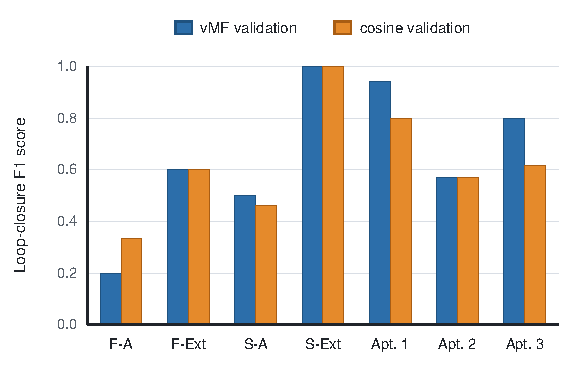
\includegraphics[width=\columnwidth]{images/vmf_cosine_comparison.pdf}
    \caption{Per-sequence loop closure $F_1$ at \qty{2}{\metre} for vMF overlap and symmetric multi-view cosine validation.}
    \label{fig:vmf_cosine_comparison}
\end{figure}

\subsection{Natural-language place retrieval}
To test the natural language experiment, we evaluate retrieval using a fixed set of $100$ English queries covering $11$ room types. The set mixes direct names, navigation commands, paraphrases, functional descriptions, visible objects, scene descriptions and indirect requests. Every query is run against each of the four annotated COLD maps, producing $400$ map--query pairs, of which $238$ contain the requested destination.

For present destinations, recall at rank one ($R@1$) and rank three ($R@3$) measure how often the correct room class appears first or among the first three nodes. Mean reciprocal rank (MRR) also rewards placing the correct class near the top. As the margin rule may leave a request unresolved, $C_{\mathrm{ret}}$ is the fraction for which it selects a candidate and $A_{\mathrm{ans}}$ is the accuracy of those selections. For absent destinations, $R_{\mathrm{rej}}$ is the fraction left unresolved. These measures separate ranking quality from the behavior of the exploratory margin rule.

Table~\ref{tab:language} reports retrieval results by sequence. When a requested room exists, its class appears among the first three nodes in $73.9\%$ of cases and appears first in $43.7\%$, and the overall MRR is $0.566$. Performance depends strongly on the building. Freiburg Extended and Saarbr\"ucken Extended exceed $0.91$ $R@3$, whereas Saarbr\"ucken A reaches only $0.548$. Direct room names give the best top-one result ($0.539$), while paraphrases ($0.381$), scene descriptions ($0.387$) and object cues ($0.409$) are harder for the system.

The relative-margin diagnostic selects $34.5\%$ of requests for existing destinations, and $57.3\%$ of those selections are correct. For missing destinations, it rejects $60.5\%$, leaving a $39.5\%$ false-selection rate. The top-two margin therefore captures how clearly one stored node outranks the others, but not whether the requested place is present in the map. The interface consequently presents ranked suggestions and requires explicit confirmation before publishing a destination. The current margin rule is therefore not reliable enough to detect absent destinations. These results display node retrieval as a useful potential application of \methodname, leaving space for future research around place confirmation and ranking improvements.

Figure~\ref{fig:nlp_examples} complements these aggregate results with four requests shown together: three visually distinctive destinations are retrieved correctly, while the large-office request exposes a plausible corridor confusion.

\begin{figure*}[!t]
    \centering
    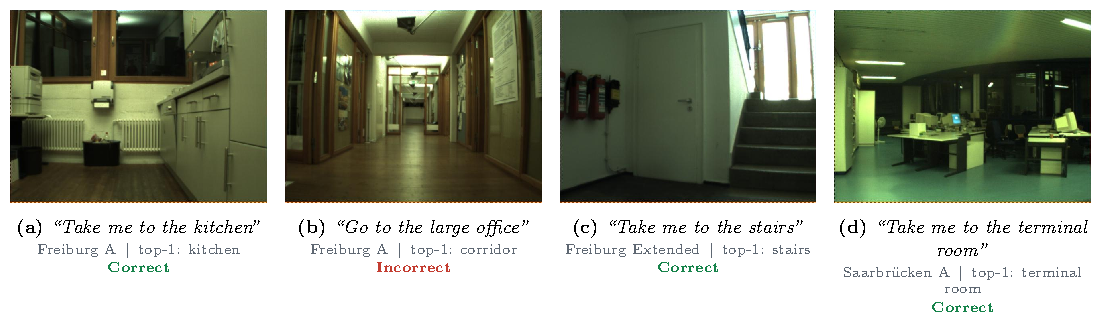
\includegraphics[width=0.98\textwidth]{images/nlp_retrieval_examples.pdf}
    \caption{Four examples of CLIP~\cite{radford2021learningtransferablevisualmodels} text-to-node retrieval. Three requests return a node of the requested room class at rank one, and the large-office request is instead matched to a corridor view.}
    \label{fig:nlp_examples}
\end{figure*}

\begin{table}[!htbp]
    \centering
    \caption{CLIP~\cite{radford2021learningtransferablevisualmodels} retrieval for 100 queries evaluated on every COLD map. The ``Present'' column gives the number of queries for which the destination is present.}
    \label{tab:language}
    \footnotesize
    \setlength{\tabcolsep}{2pt}
    \begin{tabular}{@{}lrrrrrr@{}}
    \hline
    Sequence & Present & $R@1$ & $R@3$ & $C_{\mathrm{ret}}$ & $A_{\mathrm{ans}}$ & $R_{\mathrm{rej}}$\\
    \hline
    Freiburg A              & 73 & 0.384 & 0.685 & 0.219 & 0.625 & 0.630\\
    Freiburg Extended       & 46 & 0.500 & 0.957 & 0.217 & 0.800 & 0.815\\
    Saarbr\"ucken A        & 73 & 0.384 & 0.548 & 0.370 & 0.333 & 0.519\\
    Saarbr\"ucken Extended & 46 & 0.543 & 0.913 & 0.630 & 0.690 & 0.426\\
    \hline
    Weighted                & 238 & 0.437 & 0.739 & 0.345 & 0.573 & 0.605\\
    \hline
    \end{tabular}
\end{table}

\section{Discussion}
Visual validation reduces incorrect associations at the cost of missed revisits. Its value depends on the cost of each error: an extra edge can change many graph routes, whereas a missed revisit leaves the recorded sequential route intact instead of adding a useful connection.

This interpretation relies on the uncertainty budget. Accepting a single compatible candidate assumes that the geometric phase has isolated the right place. That can be reasonable when odometry separates nearby alternatives, but a narrow gate can exclude a true revisit and a broad or misplaced gate can admit an incorrect one. The weaker-score background used in ambiguous searches relies on the same assumption. Freiburg A deserves particular attention because it contains the two false closures accepted by the complete system at \qty{2}{\metre}, and cosine validation performs better there. Both loop closures occur between nodes of adjacent rooms at the end of the trajectory, where odometry uncertainty enables the geometric gate to accept nodes farther away. This is one of the main drawbacks of this gate, especially when visual information does not provide a clear candidate.

Node creation also involves a trade-off. More boundaries improve room-transition recall and purity but split continuous visits into more segments. The adaptive detector makes node creation rates more consistent across the tested sequences, yet equal rates are not necessarily desirable in environments with different visual structure or travel speeds. Similarly, the descriptor comparison produces varying results across domains and tolerances, making it difficult to state that either of them is generally better for mapping.

The evaluation provides useful evidence about how each part of the system affects the final outcome. However, a single representative position stands in for an entire visual segment, so changing the distance tolerance can change the label of an otherwise unchanged association. Besides, endpoint proximity cannot establish traversability across walls or obstacles. With seven traversals and only 27 accepted loops in the complete configuration, a few decisions materially change the aggregate scores.

Longer deployments would also test the growth of the uncertainty budget and candidate set. The language retrieval application presents promising behavior but needs improvements in absent-destination detection and node ranking.

\section{Conclusion and Future Work}
\methodname combines adaptive spectral node creation with odometry-based candidate selection and directional sequence comparison, without task-specific training. Across seven traversals, geometric restriction reduced incorrect loop associations relative to appearance-only decisions. At a \qty{2}{\metre} tolerance, the complete system accepted 25 correct and two incorrect loops; visual validation improved precision over geometry-only association while lowering recall and $F_1$. Adaptive prominence offered a useful balance between node count and loop association, while the benefits of the visual alternatives depended on the sequence and tolerance. These findings support selective visual validation when incorrect connections are especially costly.

The next step is long-term operation on a physical robot and in larger buildings, where covariance calibration, candidate growth, and runtime can be observed under genuine drift. Reproducing the full ViT-G/14 AnyLoc configuration on GPU hardware would strengthen the retrieval baseline, while mixtures of directional distributions could represent nodes with several distinct views. The natural-language application could be improved with calibrated absence detection, independently collected and multilingual queries, and a clarification dialog before the user confirms one of the suggested destinations.

\section*{Declaration of Generative~AI and AI-assisted technologies in the writing process}
During the preparation of this work, the authors used OpenAI Codex in order to correct spelling and enhance clarity, grammar, and sentence structure. Subsequently, the authors reviewed and edited the content as needed and take full responsibility for the content of the publication.

\section*{CRediT authorship contribution statement}
\textbf{Manuel Rodriguez-Villegas:} Methodology, Software, Formal analysis, Writing – Original Draft, Visualization. \textbf{Jaime Boal:} Conceptualization, Methodology, Writing – Review \& Editing, Supervision. \textbf{Jesus Tordesillas:} Conceptualization, Methodology, Writing – Review \& Editing, Supervision.

\FloatBarrier

\balance
\bibliographystyle{elsarticle-num}
\bibliography{references}

\end{document}
